
% Environment
\documentclass[12 pt]{article}

%%%%%%%%%%%%%%%%%%%%%%%%%% Fonts 
\usepackage[english]{babel} % Multilingual package 
\usepackage[utf8]{inputenc} % Different input encoding
\usepackage{microtype} % Improves typography
\usepackage[T1]{fontenc} % Required for accented characters
\usepackage{lmodern} % Computer Modern
%\usepackage{fbb} %Use the free version of the Bembo font Family
%\usepackage{ebgaramond} % Garamond 
%\usepackage{mathptmx} % Times New Roman
\usepackage{microtype} % Typographical perfection
%\usepackage{textcomp} % Text companion fonts
%\usepackage[charter]{mathdesign} % Just for some good font...(personal taste)
\usepackage{sectsty} % Custom section fonts
%%%%%%%%%%%%%%%%%%%%%%%%% Title 
\usepackage{titling} % Maketitle and thanks commands 

%%%%%%%%%%%%%%%%%%%%%%%%% Graphics
\usepackage{graphicx} % Support for graphics
\usepackage{subfig} % Figures broken into subfigures
\usepackage{color} % Control color 

%%%%%%%%%%%%%%%%%%%%%%%%% Tables 
\usepackage{booktabs} % Nice tables
\usepackage{ltxtable} % Long tables
\usepackage{tabu} % Flexible latex tabulars
% \usepackage{threeparttable} % Clashed 
\usepackage{makecell} % Tabular column heads and multilined cells
\usepackage{multirow} % Create tabular cells spanning multiple rows 
\usepackage{array} % Extending the array and tabular environments 
\usepackage{tabularx} % Tabulars with adjustable-width columns 
\usepackage{longtable} % Long tables
\usepackage{tabulary} % Tabular with variable width columns balanced

%%%%%%%%%%%%%%%%%%%%%%%%% Text and math 
\usepackage{soul} % Hyphenation
\usepackage{bm} % Bold math
\usepackage{listings} % Inserting code
\usepackage[autostyle]{csquotes} % Double quotations
\MakeOuterQuote{"}

%%%%%%%%%%%%%%%%%%%%%%%%% Layout 
\usepackage[left=1 in,top=1 in,right=1 in,bottom =1 in]{geometry} % Page layout 
\usepackage{setspace} % Set space between lines
\usepackage{fancyhdr} % Extensive control of page headers and footers 
%\usepackage{sectsty} % Control sectional headers
\usepackage{floatrow} % Modifying the layout of floats
\usepackage{authblk} % Support for footnote style author/affiliation
\usepackage{chngcntr} % Count within sections
%\usepackage{titlecaps} % Capitalizing titles 
\sectionfont{\titlecap}

%\usepackage[nolists, %tablesfirst]{endfloat} % Move floats to the end

%\usepackage{endnotes}
%\let\footnote=\endnote
%%%%%%%%%%%%%%%%%%%%%%%%% Bibliography
% \usepackage[comma]{natbib} % Flexible bibliography
\usepackage{achicago} % Chicago style citation 
\usepackage[authordate, natbib, backend=biber,bookpages=false,doi=false,isbn=false,url=false]{biblatex-chicago}
\addbibresource{new_bibfile.bib}

%%%%%%%%%%%%%%%%%%%%%%%%% biblatex related packages 
\usepackage{lmodern}        
\usepackage{etoolbox}
\usepackage{authblk}
%%%%%%%%%%%%%%%%%%%%%%%%% Others 
\usepackage{comment} % Block commenting 
\usepackage[colorinlistoftodos]{todonotes} % Making things to do 

\usepackage[colorlinks = true,
allcolors = blue,
breaklinks=true]{hyperref}
\urlstyle{same} % URL stuff 

\usepackage[title]{appendix} % Extra control of appendices
\newcolumntype{Y}{>{\centering\arraybackslash}X}

%%%%%%%%%%%%%%% To indicate that this paper is a draft 

%\renewcommand{\maketitlehooka}{
%\vspace{-60pt}
%\raggedleft
%\small
%\fbox{Draft: Please Do Not Quote or Cite}%
%\vspace{60pt}%
%}

\makeatletter

\title{Text as Issue: Measuring Issues Preferences among Minority Groups through Ethnic Newspapers}

%\date{\today}
\date{}
\author{}
%\author{Jae Yeon Kim 
%\thanks{I thank Taeku Lee, Eric Schickler, Paul Pierson, Irene Bloemraad, Hakeem Jefferson, Jonathan Simon, Laura Stoker, Ruth Collier, Joel Middleton, Andrew McCall, Max Goplerud, and Christopher Stout for their comments. I am also grateful to Angela Yip, Brenna Uyeda, Gregory Eng, and Jenny Feng for their research assistance. This paper received the Don T. Nakanishi Award for Distinguished Scholarship and Service in Asian Pacific American Politics from the Western Political Science Association (2020).}
%\thanks{Direct correspondence to Jae Yeon Kim, Department of Political Science, 210 Barrows Hall #1950, Berkeley, CA 94720, E-mail: jaeyeonkim@berkeley.edu}
%\thanks{All replication files can be found at https://github.com/jaeyk/content-analysis-for-evaluating-ML-performances}
%}

\begin{document}

\maketitle       

\singlespacing

\begin{abstract}
\noindent 
Survey research has been central to studying racial and ethnic politics in the US. However, most of these surveys were developed in the 1990s and 2000s, so they are not useful if researchers are interested in historical questions. The text-as-data approach provides a solution to this problem by turning ethnic newspaper articles into data. In this study, I present a mixed-method framework that combines a case selection strategy, content analysis, and text classification to utilize a large collection of ethnic newspaper articles for descriptive inference. As a demonstration of this framework, I apply machine learning techniques to 78,383 articles from Asian American and African American newspapers from the 1960s through the 1980s. Content analysis assesses data quality by measuring what and how human coders label the training data. Text classification demonstrates that Asian American newspapers issued linked progress articles by 110\% more than African American newspapers did. By contrast, African American newspapers produced linked hurt articles by 133\% more than Asian American newspapers did. The gap between the two groups widened up to 10 times when the training data were measured by the minimum rather than the maximum threshold.
\end{abstract}

\thispagestyle{empty}

\makeatletter
\clearpage

\pagenumbering{gobble}
\pagenumbering{arabic}

\doublespacing

Racial and ethnic politics in American politics has evolved based on the development of new surveys. The American National Election Studies (ANES) consists of high-quality panel data that go back to 1948 and have been central in investigating public opinion in American politics \citep{campbell1980american, zaller1992nature, bartels1999panel}. However, when it comes to studying the politics of ethnoracial minority groups, the data have clear limitations because these groups take up only a very small portion of ANES data \citep{conway2004politics}. Other prominent panel data on public opinion, such as the General Social Survey (GSS), are no exception. Racial and ethnic politics researchers have tried to overcome this data limitation by creating new surveys. To name a few, the National Black Election Study\footnote{For more information, see \url{https://www.icpsr.umich.edu/icpsrweb/ICPSR/series/163.}} was developed in 1984, the Latino National Political Survey\footnote{For more information, see \url{https://www.icpsr.umich.edu/icpsrweb/ICPSR/studies/6841.}} in 1989, the National Surveys of Latinos\footnote{For more information, see \url{https://www.pewresearch.org/topics/national-survey-of-latinos/.}} in 2002, the Pilot National Asian American Political Survey\footnote{For more information, see \url{https://www.icpsr.umich.edu/icpsrweb/ICPSR/studies/3832.}} in 2000 and its official version\footnote{For more information, see \url{https://naasurvey.com/data/.}} in 2008, and the Comparative Post-Election Survey\footnote{For more information, see \url{https://cmpsurvey.org/.}} in 2008. This new stream of data has enabled a large number of research to be conducted in African American, Latino, and Asian American politics \citep{gurin1990hope, tate1993protest, dawson1994behind, fraga2011latinos, wong2011asian, mcclain2018can}. Nevertheless, most of these surveys are short lived and thus not comparable to the ANES or GSS in terms of longevity. More importantly, these surveys were mostly developed in the 1990s and 2000s, so they are not useful if researchers are interested in historical questions, such as the political origins and development of minority political movements. For instance, the 1960s and 1970s were the pinnacles of minority political activism in the US. Yet, because of data limitation, the investigation of this critical period has been left to anecdotal examples \citep{munoz1989youth, wei_asian_1993, joseph2006black, maeda2012rethinking, ishizuka2016serve, linder2018text}. 

The text-as-data approach provides a solution to this long-standing problem in the study of racial and ethnic politics in the US. This approach expands the data infrastructure in racial and ethnic politics by turning ethnic newspaper articles into data. Ethnic newspapers have been an essential part of mobilization networks for ethnoracial minority groups. Because mainstream media did not cover minority issues, minority activists founded ethnic newspapers to develop their own political agendas and discuss their unique political issues \citep{le1992asian, dawson1994black, rodriguez1999making, dawson2001black, kannegaard2008press, harris2010barbershops}. Therefore, ethnic newspapers are invaluable historical resources to fill gaps in the quantitative analysis of US racial and ethnic politics---they trace prevalent issues and how these tendencies varied between ethnoracial minority groups over time. Traditionally, content analysis was the main means to analyze newspaper articles; researchers manually collected, read, and interpreted these documents. Large-scale text analysis was impossible until modern computational techniques, such as web scraping, natural language processing, and machine learning, automated the labor-intensive data collection and analysis process \citep{grimmer2013text, wilkerson2017large}.

Nevertheless, more is not always better. The advantage of large-scale computational text analysis over traditional content analysis is scale. A large sample has some nice features for hypothesis testing because it reduces the size of standard errors and establishes the law of large numbers (or the central limit theorem). However, because newspaper articles are collected through non-probability sampling, the large size of the data may also increase the degree of bias in them \citep[685-688]{meng2018statistical}. For instance, not all ethnic newspapers made their records public, not to mention digitized. Because these decisions would have been influenced by the financial status of such newspapers, among other factors, the collection of these newspaper articles would have non-random missing data and would likely not be representative. 

Furthermore, measuring issues that appear in ethnic newspaper articles is difficult. These issues could be conceptualized and measured at a high (meta issues) or low level (specific issues). Meta issues or broad issue frames are useful in text classification, a supervised machine learning technique. Reducing the number of classes that need to be classified increases the number of observations for each class, which is the volume of training data. Furthermore, a small number of classes simplify the coding scheme for human coders and lower their cognitive loads, thus enhancing the reliability of the training data \citep{mikhaylov2012coder}. Nevertheless, these meta issues are conceptually valid only if they are closely associated with specific issues they are supposed to represent. More importantly, different thresholds could be applied to label training data. The minimum threshold indicates that at least one human coder must agree with the coding decision. The maximum threshold indicates that all human coders must agree with the coding decision. These different thresholds may influence machine learning outcomes by providing different qualities of training data. The maximum threshold produces more reliable training data because it is based on strictly consistent coding decisions among human coders. 

In response to these methodological and conceptual challenges, I present a mixed-method framework that combines a case selection strategy, content analysis, and text classification. This framework helps utilize a large collection of ethnic newspaper articles for descriptive inference. The key idea is that computational text analysis techniques build upon and never replace human decisions \citep[268]{grimmer2013text}. Technical guidelines exist for the automated part of the text analysis process, such as preprocessing documents, training algorithms, and evaluating their performance. Yet scholars have rarely engaged with how data collection and measurement decisions---humans in the machine learning loop---affect machine learning outcomes \citep{mikhaylov2012coder, gitelman2013raw, geiger2020garbage}. The framework addresses this problem by structuring data collection and demonstrating the sensitivity of machine learning outcomes to measurement decisions. 

As a demonstration of this framework, I apply machine learning techniques to 78,383 articles from Asian American and African American newspapers from the 1960s through the 1980s. I intentionally selected Asian American and African American newspapers based on the West Coast because Asian Americans and African Americans in the region shared strong social and political networks during the period under investigation. The case selection strategy reduces alternative explanations. Meta issues among ethnoracial minority groups in the US could be divided into two categories: providing collective gains (linked progress issue) and preventing collective losses (linked hurt issue). Content analysis assesses data quality by measuring what and how human coders label the training data. Text classification demonstrates that Asian American newspapers issued linked progress articles by 110\% more than African American newspapers did. By contrast, African American newspapers produced linked hurt articles by 133\% more than Asian American newspapers did. The gap between the two groups widened up to 10 times when the training data were measured by the minimum rather than the maximum threshold. 

This study makes several contributions. Substantially, the findings deepen the understanding of why building interracial coalitions has been difficult in the US \citep{kaufmann2003cracks, rogers2006afro}. Historians of US race relations have pointed out preference misalignment as a hurdle to the formation of interracial coalitions \citep{brilliant2010color, kurashige2010shifting}. The study presents the first systematic evidence of the magnitude of this problem by using a large-scale computational text analysis. Although the evidence is purely descriptive, it provides new theoretical insights into the dynamics of interracial coalition building in the US. Methodologically, the study demonstrates why content analysis, ensuring the quality of training data, is vital in machine learning applications. Using less reliable data leads to not only less accurate predictions but also more extreme interpretations. Machine learning has a strong potential to expand data infrastructure in political science by making the collection and analysis of large-scale data efficient. This feature is especially attractive for a data-hungry field, such as racial and ethnic politics. However, in using this method for knowledge accumulation, acknowledging its limitation is equally crucial. This powerful method reaches its potential only if the quality of training data is not compromised. Examining data quality is essential in using the text-as-data approach for political science research to reassure the credibility of prediction results and interpretations.

\section{Conceptualization}

Historically, ethnoracial minority groups have been subject to discrimination in the US \citep{chae2008unfair, hwang2008impact, rothstein2017color, trounstine2018segregation, reardon2019geography, williams2019racism}. Meta issues among them are the broad frames that define relevant issues to cope with unfair treatments. \citet{dawson1994behind} tackled this conceptual problem in his analysis of the source of Black political solidarity. His Black utility heuristic theory argued that the long experience of racial discrimination makes it difficult for African Americans to separate their individual utility from group utility. He called the connection linked fate and demonstrated how this utility heuristic accounts for the strong groupness of African American political behavior.

I follow his footsteps but also take one step further by differentiating the mechanisms that produce linked fate. Taking this step is useful to generalize Dawson's framework and measure how issue priorities between minority groups vary not only in degree but also in kind. Based on Dawson's theorizing, linked fate as a psychological construct at $t_{2}$ is influenced by sociological processes at $t_{1}$. The sharing of issue frames through ethnic newspapers is one of such mechanisms \citep[56-61]{dawson1994behind}. It helps group members recognize the issues that are relevant and deserve their attention \citep[1058]{nelson1996issue}. Ethnic newspapers perform this function by framing issues in the following two ways: 

\begin{itemize}
\item Linked progress frame: emphasizing the positive connection between individual and group utility or promoting collective gains 
\item Linked hurt frame: highlighting the negative connection between individual and group utility or preventing collective losses 
\end{itemize}

I define ethnic newspaper articles by using the linked progress frame as linked progress articles. In a similar vein, I define ethnic newspaper articles by using the linked hurt frame as linked hurt articles. Because linked progress and hurt are not exclusive categories, some ethnic newspaper articles might be classified as both linked progress and hurt articles.

\section{Theory}
I propose a simple theory that explains how ethnic newspapers decide the relative production of linked progress and hurt articles. Because ethnic newspapers rely on the ethnic niche market, many of them struggle financially and issue articles selectively. Ethnic newspapers issue a specific article type only if it would advance or protect their group interests. Government policies are the key factors that influence these calculations. Beneficial government policies enhance expected group gains. Oppressive government policies increase expected group losses. When a group faces the risk of not being able to take full advantage of beneficial policies, an ethnic newspaper aligned with the group would issue more linked progress articles to raise awareness of these opportunities among the group members. When the same group is confronted with the risk of being targeted by oppressive policies, an ethnic newspaper aligned with the group would issue more linked hurt articles to alarm the group members regarding these threats. Table \ref{tab:expectations} summarizes these theoretical expectations.

\begin{table}[htbp!]
	\centering
	\caption{How ethnic newspaper produce linked progress and hurt articles in response to government policies}
	\label{tab:expectations}
	\begin{tabularx}{\textwidth}{ X | X | X}
		\toprule
		 & Strong beneficial government policies & Weak beneficial government policies \\ \midrule
		Strong oppressive government policies & Increase the mix of linked progress and hurt articles & Increase linked hurt articles \\ \hline
		Weak oppressive government policies & Increase linked progress articles & None \\ \hline 
		\bottomrule
	\end{tabularx}
\end{table}

\section{Hypotheses}

We can draw the following two observable implications from the theory. If a minority group is exposed to beneficial government policies, the newspaper aligned with the group would issue more linked progress articles. If a minority group is exposed to oppressive government policies, the newspaper aligned with the group would issue more linked hurt articles. Suppose that for class “Linked progress” and class “Linked hurt,” 1 denotes membership in the class and 0 the opposite. $P(\textrm{Meta issue type} = 1|\textrm{Government policy type})$ indicates the probability of an ethnic newspaper issuing an article using a particular type of meta issue ($\in \textrm{\{Linked progress, Linked hurt\}}$) given that the group the newspaper is aligned with is exposed to a specific type of government policy ($\in \textrm{\{Beneficial, Oppressive\}}$). We can formally define the hypotheses as follows:

\begin{itemize}
    \item Hypothesis 1:  $P(\textrm{Linked progress} = 1|\textrm{Beneficial government policies}) > \\
    P(\textrm{Linked hurt} = 1 | \textrm{Beneficial policies})$
    \item Hypothesis 2: $P(\textrm{Linked hurt} = 1| \textrm{Oppressive government policies}) > \\
    P(\textrm{Linked progress} = 1 | \textrm{Oppressive government policies})$. 
\end{itemize}

\section{Case Selection}
Ethnic newspaper articles are an instance of found data. Unlike designed data, such as experimental or survey data, found data are a kind of data in which researchers are not involved in the design of the data collection process \citep[82]{salganik2019bit}. For this reason, knowing the sampling frame and estimating the extent to which the sample, the available newspaper articles, are biased are almost impossible. Nevertheless, found data are useful for testing historical mechanisms because scaling up the collection of found data is manageable. Designing and implementing several rounds of surveys or experiments are quite expensive. Collecting a large number of existing records over a long period is relatively cheap because by definition, researchers did not create these data. In the theory proposed above, variations in the outcomes are created by policy changes, which occur slowly. Therefore, testing theoretical implications requires long-term observations. 

For hypothesis testing, ideally, we would like to compare a set of ethnic newspaper articles about two groups that are exactly alike, except that one group is relatively exposed to beneficial policies and the other group is relatively exposed to oppressive policies. Unfortunately, no such identical cases exist in the real world \citep[947]{holland1986statistics}. The next best option is to find cases in which the characteristics of the two minority groups are as similar as possible, except for their differential policy treatments. In-depth case knowledge helps identify these well-matched cases.

Asian Americans and African Americans on the West Coast are two of the most similar historical cases exposed to divergent policy treatments. Both groups were subject to racial discrimination on the West Coast for decades. Racial discrimination against Asian Americans started in the late 19th century by “a white supremacist alliance in Congress”---southern Democrats and western Republicans \citep[88]{king2005racial}. The Chinese Exclusion Act of 1882 singled out the Chinese as the first racially excluded group by immigration policy in the US \citep{lee2003america, ngai2014impossible}. The immigration ban was extended to all other Asian national origin groups through the Immigration Act of 1924, although Filipinos were exempted because of their American national status. Similarly, the California Alien Land Law of 1913 deprived Asian Americans of their property rights except those with birthright citizenship. Racial discrimination against African Americans soon appeared in the region as a large number of African Americans moved to the West during the Second Great Migration. For instance, housing discrimination against African Americans established a rigid color line between African American and White neighborhoods in the East Bay of the San Francisco Bay Area \citep{self2005american}. Even though booming industrial cities on the West Coast, such as Los Angeles, provided unprecedented economic opportunities to African Americans, the postwar economy had a clear racially charged hierarchical structure \citep{sides2006city}. 

More importantly, the physical and social boundaries between African American and Asian American neighborhoods on the West Coast were permeable. When African Americans moved to the West during World War II, they found a rare housing opportunity among vacant houses created by the internment of Japanese Americans. For this reason, from Los Angeles to Seattle, African American neighborhoods were located directly next to Asian American ethnic enclaves. The proximity may also explain why and how the Black Power and the Asian American movements co-evolved in inner cities in the West Coast \citep{prashad2002everybody, maeda2005black, ho2008afro, maeda2012rethinking, ishizuka2016serve, watkins2012black}. The Red Guard Party, a radical Asian American organization founded in San Francisco in 1969, was modeled on the Black Panther Party established in Oakland across the Bay in 1966. Like the Black Panther Party, the Red Guard Party had a 10-point program and ran a free breakfast program, and their members wore berets \citep[1079-1089]{maeda2005black}. 

Despite close social and political networks, Asian American and African American political movements emerged in parallel and did not coalesce into a coalition among people of color. Student activists of color focused on racial justice were certainly present on college campuses \citep{umemoto1989strike, wei_asian_1993, maeda2012rethinking}. Nonetheless, outside college campuses, counterexamples abound \citep[238-240]{brilliant2010color}. Interracial coalitions that emerged on college campuses were an exception rather than a rule. When these activists became involved in communities and attempted to make differences for marginalized members, they would not attempt to influence policies that did not directly affect the welfare of their community members over the ones that had more direct impacts because they were deprived of political resources. The occasional rainbow coalition building efforts did not last because these groups had discordant priorities in realizing racial justice.

Recent historical studies and my own archival research show how the wide spectrum of policies introduced in the 1960s created the source of the discord. President Lyndon B. Johnson expanded both oppressive and beneficial policies in the 1960s, and these policies raised different kinds of challenges for African Americans and Asian Americans. Although Richard Nixon has been credited for spearheading the War on Crime in the US, a recent historical study revealed that the seed of mass incarceration had already been sown by Lyndon B. Johnson. Johnson expanded federal assistance in militarizing policing through the establishment of the Office of Law Enforcement Assistance in 1965. He stated that the US government was simultaneously engaging in two wars---the war in Vietnam and that in inner cities in the US---and described urban police officers as frontline soldiers fighting “a war within our boundaries” \citep[102-105]{hinton2015war}. For African American migrants from the South who then settled in the West, these punitive government policies were nothing but familiar. When African American activists protested about the wrongful convictions of three African American inmates at California's Soledad Prison in 1970, they rallied around the following slogan: “Save the Soledad Brothers from Legal Lynching” \citep{davis1971soledad}. As oppressive government policies disproportionately targeted African Americans, African American newspapers tried to alarm their group members regarding these threats and mobilize them in order to protect their group's rights to be safe and alive. 

Asian Americans wrestled with a different kind of policy challenge. The Immigration and Naturalization Act of 1965 resumed mass immigration from Asia. During the first wave of mass Asian immigration, the majority of Asian immigrants were cheap laborers. This time was different; the new wave of immigrants included middle-class and educated people. Housing discrimination against Asian Americans weakened as the Cold War began, and some Asians, especially Chinese Americans, were considered allies \citep{brooks2009alien}. Taking advantage of this trend, these well-off Asian Americans bypassed the run-down old ethnic enclaves in inner cities and built new ethnic hubs in suburban areas \citep{kwong1996new, lai2003downtown, li2006urban, zhou2010chinatown}. Consequently, those left behind in the old Chinatown, Japantown, and Manilatown suffered from deteriorating neighborhood conditions and desperately needed outside support. Johnson's other domestic political agenda, the War on Poverty programs, provided the kind of support that Asian American activists in these communities sought but with one serious limitation. From the perspective of government officials, Asian American communities were too small and fragmented \citep{kuramoto1976lessons}. This condition made them a less-ideal subject of federal social policies, as the cost of delivering service to them was too high and the total number of people served by the program was too small. Michio Suzuki, deputy commissioner of the Administration for Public Services in Washington D.C., warned Asian American social service providers that they should “act together” because federal officials were unhappy when they had to fund various Asian groups separately as a result of the lack of coordination between them (\textit{International Examiner}, 30 April, 1979).\footnote{\textit{International Examiner} is a free bi-weekly Asian American community newspaper based in Seattle. I will describe this newspaper in detail in the data section.} After decades-old exclusion from the state's social protection, Asian Americans at last received an opportunity to gain access to government resources. Yet federal grant makers did not recognize them as a viable minority group. Asian American newspapers tried to raise awareness of these opportunities among their group members in order to advance their group's interests. 

The structured case comparison helps reduce alternative explanations, such as neighborhood backgrounds or political ideologies. Nevertheless, some unobserved differences between the groups remain, and they might have influenced the relative production of linked progress and hurt articles by Asian American and African American newspapers. For this reason, this approach is not suitable for causal inference. Rather, the aim of this case selection is mainly to strengthen descriptive inference from a large-scale collection of ethnic newspaper articles.

\section{Data}

Of the many newspapers and magazines written by and for Asian Americans and African Americans, I use the records of \textit{Asian Week} (1983-1989), \textit{International Examiner} (1976-1987), \textit{The Sun Reporter} (1968-1979), \textit{The Oakland Post} (1968-1981), and \textit{The Sacramento Observer} (1968-1975). I selected these newspapers because they were all founded in inner cities on the West Coast, devoted substantial pages to describing community affairs, and frequently shared news about community organizations in the area. 

\textit{International Examiner}, founded in Seattle in 1974, and \textit{Asian Week}, based in San Francisco in 1979, were the two leading Asian American newspapers on the West Coast. Unlike other Asian ethnic newspapers that catered to national origin groups (e.g., Chinese, Japanese, Filipinos), these newspapers aimed to represent the united voice of Asian Americans.

\textit{Asian Week} was the first English-language Asian American publication and the largest until it closed in 2012 \citep[29-31]{ling2015asian}. The newspaper closely followed news related to local community-based organizations and paid special attention to the growing involvement of Asian Americans in electoral politics. \textit{International Examiner} is the oldest and largest non-profit Asian American newspaper in the Northwest. It was founded by two local business persons and then---because of financial failure---sold to the Alaska Cannery Workers Association, a local labor union for Filipino migrant workers, for \$1 in 1975. Afterward, \textit{International Examiner} operated as a free biweekly newspaper with a focus on community activism among Asian Americans. One of the first issues published after its acquisition was an article on the activities of the Committee for Corrective Action Program, a coalition of Asian American activists and organizers in the International District. Similarly, the newspaper brought community organizers, such as Robert Santos, director of Inter*Im, a housing advocacy organization, and Donnie Chen, director of the International District Emergency Center, as regular contributors (\textit{International Examiner} 15 June 1983). 

Similar to its Asian American counterpart, the African American corpus in the data was politically progressive. \textit{The Sun Reporter} was founded in San Francisco in 1944 as the city's first Black press. The founder, Dr. Carlton B. Goodlett, was an African American civil rights activist and former president of the local branch of the National Association for the Advancement of Colored People. Thomas Fleming, who worked as an editor, reporter, and columnist for the newspaper for 61 years from its founding, also held a strong political commitment to racial justice. He once argued that the mission of the Black press was to serve as “the watchdogs” in order to guarantee the constitutionally granted citizenship status of “former chattel slaves” (\textit{Sun Reporter} August 2, 1975). \textit{The Oakland Post} was founded in 1963 and was politically less vocal, as the newspaper intentionally focused on not “making a social statement” but instead “just covering the news” to increase its readership and thus its impact (\textit{The Oakland Post} February 15, 1981). Nevertheless, as Oakland was a main center of African American political mobilization on the West Coast, it was almost impossible for the newspaper not to address the topic of racial justice. Between 1968 and 1981, the newspaper covered The Black Panther Party 192 times. \textit{The Sacramento Observer} was founded in Sacramento in 1962 and supported the Sacramento Urban League and the Sacramento Area Black Law Caucus. The newspaper also played a particularly important role in informing and alerting the African American community in Sacramento about the development of the Civil Rights and the Black Power Movements in other parts of the country \citep[25]{covin2009black}.

I downloaded data from these five newspapers from the Ethnic NewsWatch database, which has compiled more than 2.5 million articles published in US ethnic newspapers and magazines.\footnote{For more information, see \url{https://www.proquest.com/products-services/ethnic_newswatch.html.}} ProQuest created this database and does not allow web scraping. However, one can still download articles and save them as hypertext markup language (HTML) files. I have turned these HTML files into a single dataset by using the Beautiful Soup library in Python. Other key African American newspapers on the West Coast, such as \textit{Los Angeles Sentinel}, were not included, as the only articles published by that newspaper after 1991 were available in the database. At first, there were more than 80,000 articles. In the data-cleaning process, I discovered that data from \textit{The Sun Reporter} from early 1973 to late 1974 did not include the complete articles, only their abstracts. For this reason, I omitted such data. This reduced the total number of articles to 78,383. Table \ref{tab:} summarizes the number of newspaper articles in the corpus.

\begin{table}[htbp!]
\centering
\begin{tabularx}{\linewidth}{X|X|X|X|X|X}
\toprule
Title & Asian Week & The International Examiner & The Sun Reporter & The Oakland Post & The Sacramento Observer \\
\midrule 
Period & 1983-1989 & 1976-1987 & 1968-1979 & 1968-1981 & 1968-1975\\
\midrule
N & 11,883 & 2,719 & 24,793 & 29,560 & 9,428\\
\bottomrule
\end{tabularx}
\caption{\label{tab:}Number of each newspaper articles in the corpora}
\end{table}

\section{Empirical Strategies}
The goal of the empirical strategy was to find a systematic and cost-efficient way to measure every article based on the conceptual framework proposed above. I achieved this goal by combining content analysis and text classification. Content analysis, a systematic description of the content of communication \citep[18]{berelson1952content}, is important for assessing the quality of training data. Labeling over 78,000 articles is a very labor-intensive process. Even if labeling a single article took only one minute, labeling 78,383 articles would have required 1,305 hours, assuming human coders never sleep, eat, or take a break. If the same task were performed by machine learning algorithms, it would only take several minutes. However, automated text classification needs supervision. What machines do is mimic human behaviors. Because the machine can only follow where humans lead, the quality of human coding influences the quality of automated text classification. For instance, human-labeled training data with low reliability may increase noise and lead to the low accuracy of predicted labels. Therefore, assessing the quality of human coding is crucial to providing baseline estimates for machine learning performance. Figure \ref{fig:workflow} describes the workflow from selecting cases to testing the hypotheses.

\begin{figure}[htbp!]
    \centering
    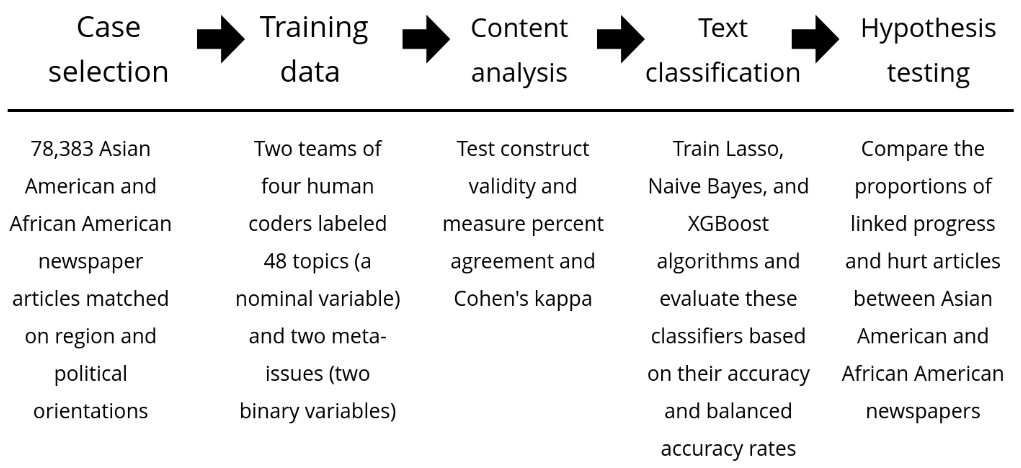
\includegraphics[width=1\linewidth]{workflow.png}
    \caption{Workflow}
    \label{fig:workflow}
\end{figure}

\subsection{Training Data}
I hired four undergraduate research assistants and labeled the training data based on the following procedures. The human coders labeled two meta issues and a list of topics because these topics are useful for testing construct validity. Throughout these procedures, none of the human coders were informed about the research hypotheses.

\begin{enumerate}
    \item Detecting topics and distributing articles: I employed topic modeling using the stm package in R \parencite{roberts2014structural} to inductively discover topics from each newspaper.\footnote{Topic modeling is sensitive to initialization. The stm package uses spectral initialization as a default option because it produces globally consistent or stable outcomes under reasonable assumptions \citep[10]{roberts2014structural}} I randomly divided these topics (N = 48) into two parts and assigned 100 articles from each topic in the first part to one team of two human coders and 100 articles from each topic in the second part to another team. I asked the human coders to label each topic based on these articles without consulting the other team member. 
    \item Topic labeling: The two teams spent two weeks labeling topics and then another week agreeing on the common labels through intergroup discussions. In the process, the human coders created a list of topics related to the articles. 
    \item Meta issue labeling: After the topic labeling, I randomly selected 1,008 articles from the Asian American corpus and 1,008 articles from the African American corpus stratifying on the year variable. Year was selected as a stratifying variable because key issues may change over time. I then paired the human coders into two groups again and assigned one group to the Asian American corpus sample and the other group to the African American corpus sample. The human coders were not aware of the hypotheses the research attempts to test. Each team coded whether the articles in the sample were about promoting collective gains (yes = 1, no = 0) or preventing collective losses (yes = 1, no = 0). The process created two binary variables---collective gain and collective loss. I do not create one binary variable and use linked progress and hurt as its two exclusive classes because this ignores mixed or none classes identified in Table \ref{tab:concet_map}. Creating two separate binary variables is a more reasonable approach. In doing so, the human coders also labeled each article with a relevant topic from the list they created in step 2.
\end{enumerate}

\begin{table}[htbp!]
	\centering
	\caption{Conceptual Matrix}
	\label{tab:concet_map}
	\begin{tabularx}{\textwidth}{ X | X | X}
		\toprule
		& Linked progress & Non-linked progress \\ \midrule
		Linked hurt & Mixed & Exclusive linked hurt \\ \hline
		Non-linked hurt & Exclusive linked progress & None \\ \hline
		\bottomrule
	\end{tabularx}
\end{table}

\subsection{Content Analysis}
I assessed the quality of the human-labeled training data by using three criteria. The first two criteria are for measuring inter-coder reliability, and the last one is for measuring construct validity.

\begin{itemize}
    \item Percentage agreement measures the percentage of the agreed coding decisions made by pairs of coders. The calculation of percentage agreement is fairly simple. Suppose two human coders measure a binary variable. Subtracting the values recorded by coder 1 from the values recorded by coder 2 returns some 0s. The number of 0s divided by the number of units provides the percentage agreement \citep[278]{mchugh2012interrater}. Therefore, percentage agreement is an intuitive method to assess the accuracy of human coding. Nevertheless, it is also a crude one, as it does not account for a certain degree of agreement that would simply arise by chance. Several studies have demonstrated how this measure tends to overestimate the true agreement among human coders \citep{birkimer1979back, suen1985effects, lombard2002content}. 
    \item Cohen's kappa coefficient provides measures for the degree of reliability in inter-coder agreement. Suppose $p_{a}$ indicates the proportion of actual agreement and $p_{e}$ the proportion of chance agreement. The difference between the two quantities, $p_{a} - p_{e}$, represents the proportion of units in which the agreement occurred beyond chance. $1-p_{e}$ represents the remaining units when the chance agreement is excluded \citep[39-40]{cohen1960coefficient}. The coefficient ($k$) or kappa is defined as 
    
    \begin{equation}
    k = \frac{p_{a} - p_{e}}{1 - p_{e}} 
    \end{equation}
    
   The kappa can range from -1 and +1 and 0. In practice, a kappa smaller than or equal to 0 indicates no agreement, a kappa in the 0.01-0.02 range indicates slight agreement, a kappa in the 0.21-0.40 range indicates fair agreement, a kappa in the 0.41-0.60 range indicates moderate agreement, a kappa in the 0.61-0.80 range indicates substantial agreement, and a kappa in the 0.81-1 range indicates an almost perfect agreement \citep[279]{mchugh2012interrater}. The key point is that a high kappa score is desirable because it represents a low degree of faulty evidence in the training data. I also check whether the kappa score increases when I exclude the articles covering non-political topics in the training data because these articles could confuse human coders and decrease inter-coder reliability.
    \item Construct validity is about whether the measures measure what they are supposed to measure based on the underlying theory \citep{cronbach1955construct}. At the conceptual level, linked progress and hurt labels and topic labels are closely associated because the meta issues should represent these topics. Articles labeled as linked progress are expected to cover topics on supportive government policies (convergent validation) more likely than oppressive government policies (discriminant validation). Articles labeled as linked hurt should behave in an opposite way \citep{campbell1959convergent}. I test these assumptions by calculating the difference between the number of linked progress articles and that of linked hurt articles associated with particular topics. 
    \item Finally, I examine the relationship between reliability and construct validity by examining how these differences vary by measurement decisions. At the minimum, articles could be defined as linked progress or linked hurt if one of the two human coders said so (minimum threshold). At the maximum, articles could be defined as such if all the human coders agreed (maximum threshold). The minimum threshold is a naive approach, and the maximum threshold provides more reliable data.
\end{itemize}

\subsection{Text Classification}
Using the labeled articles, I trained and tested the least absolute shrinkage and selection operator (Lasso), naive Bayes, and extreme gradient boosting (XGBoost) algorithms. Textual data are high-dimensional data because the number of features (e.g., words) is far greater than the number of documents. Lasso reduces this high number of features in an interpretable and stable way by shrinking some coefficients in absolute value and setting others to 0 \citep[267-273]{tibshirani1996regression}. Naive Bayes is naive because it assumes that the effect of a feature ($X$) on a class ($C$) or $P(C|X)$ is independent of the effects of other features \citep[410]{maron1961automatic}. Despite this strong conditional independence assumption, the naive Bayes classifier has been proven successful in automated text classification \citep[11-12]{maron1961automatic} because when the dependencies among features are distributed evenly across classes, the naive Bayes classifier could still be optimal \citep{zhang2005exploring}. XGBoost is a relatively recently developed algorithm that has demonstrated high performance in many machine learning competitions. Boosting improves machine learning performance by incrementally combining the performance of many weak classifiers \citep{freund1999short, friedman2000additive}. Gradient boosting is a flexible version of this approach \citep{breiman1997arcing, mason2000boosting, friedman2001greedy}, and XGBoost helps apply it to large-scale data efficiently \citep{chen2016xgboost}. I put 70\% of the sample articles into the training set and the rest into the test set by using the scikit-learn library in Python, again stratifying on the year variable. 

For the pre-processing, I tokenized the documents, removed special characters and white space, and turned these tokens into lower case. For the feature extraction, I used the bag-of-words model \citep{harris1954distributional}. It is a simple representation of the text because it only counts word frequencies in each article. These term frequencies are used as features to train algorithms and make predictions. I only used the top 5,000 most frequently appearing terms because Zipf's law expects frequently appearing features in documents to be a small fraction \citep{zipf1936psycho, zipf1949human}. The rest of the features will only increase sparsity in the training data and slow down the algorithmic process. I also construct n-gram, a sequence of n items from a document, with a maximum length of two, because some key words, such as “civil rights,” are sensible in bigrams.

I evaluate machine learning performance by examining accuracy and balanced accuracy rates. In a binary classification problem, machine learning performance is measured by a confusion matrix. A correctly predicted positive class is a true positive (TP), whereas an incorrectly predicted positive class is a false positive (FP). A correctly predicted negative class is a true negative (TN), whereas an incorrectly predicted negative class is a false negative (FN). The accuracy rate of a binary classifier is defined as $\frac{TP + TN}{TP + FN + TN + FP}$. This plain accuracy rate is not ideal when the training data suffer from a class imbalance problem. The algorithm is then likely to perform worse for the minority class than the majority class. This problem, however, could be unnoticed if the classifier works well in predicting the majority class. Consider the hypothetical case presented in Table \ref{tab:evaluations}. The training data are imbalanced because the size of the positive class is 10 and the size of the negative class is 90. The algorithm failed to predict the positive class. Despite this, because the negative class was predicted perfectly, the accuracy rate was 90\%. Nevertheless, if one looks at other scores, the performance is far less promising. Whereas the true negative rate (or specificity) is 100\%, the true positive rate (or sensitivity) is 0. If the true positive rate (correctly labeling linked progress and hurt articles) is critical for hypothesis testing, then this situation should be avoided. The balanced accuracy rate, which averages specificity and sensitivity, is a more robust measure. The balanced accuracy rate of a binary classifier is defined as $\frac{1}{2}(\frac{TP}{P} (Sensitivity) + \frac{TN}{N} (Specificity))$ \citep[3122-3123]{brodersen2010balanced}. The absolute difference between the two measures shows the effect of imbalanced training data on prediction accuracy. If the difference is substantially large, I address this problem by randomly oversampling the minority class in the training data with replacement (upsampling) and examining performance improvement using the accuracy and balanced accuracy rates. I also check the extent to which the machines performed better or worse than the human coders by comparing the percentage agreement and the two machine learning performance measures. I select a classifier that shows stable high performance \citep{yu2013stability}, I predict the unlabeled data, and I test the hypotheses by comparing the proportion of linked progress and hurt articles in the Asian American and African American corpora.

\begin{table}[htbp!]
	\centering
	\caption{Hypothetical imbalanced training data}
	\label{tab:evaluations}
	\begin{tabularx}{\textwidth}{ X | X | X}
		\toprule
		 & Predicted positive & Predicted negative \\ \midrule
		Positive class & Number of TP results: 0 & Number of FN results: 0 \\ \hline
		Negative class & Number of FP results: 10 & Number of TN results: 90 \\ \hline 
		\bottomrule
	\end{tabularx}
\end{table}

\section{Content Analysis}

\subsection{Percentage Agreement}
To begin with, the percentage agreement displays the high reliability of the labels. Figure \ref{fig:percentage_agreement} shows that the inter-coder agreement reached 88\% for the linked hurt articles in both the African American and Asian American corpora. The metric is slightly lower for the linked progress articles: 7\% down for the African American newspaper and 8\% down for the Asian American one. However, this difference is marginal.

\begin{figure}[htbp!]
    \centering
    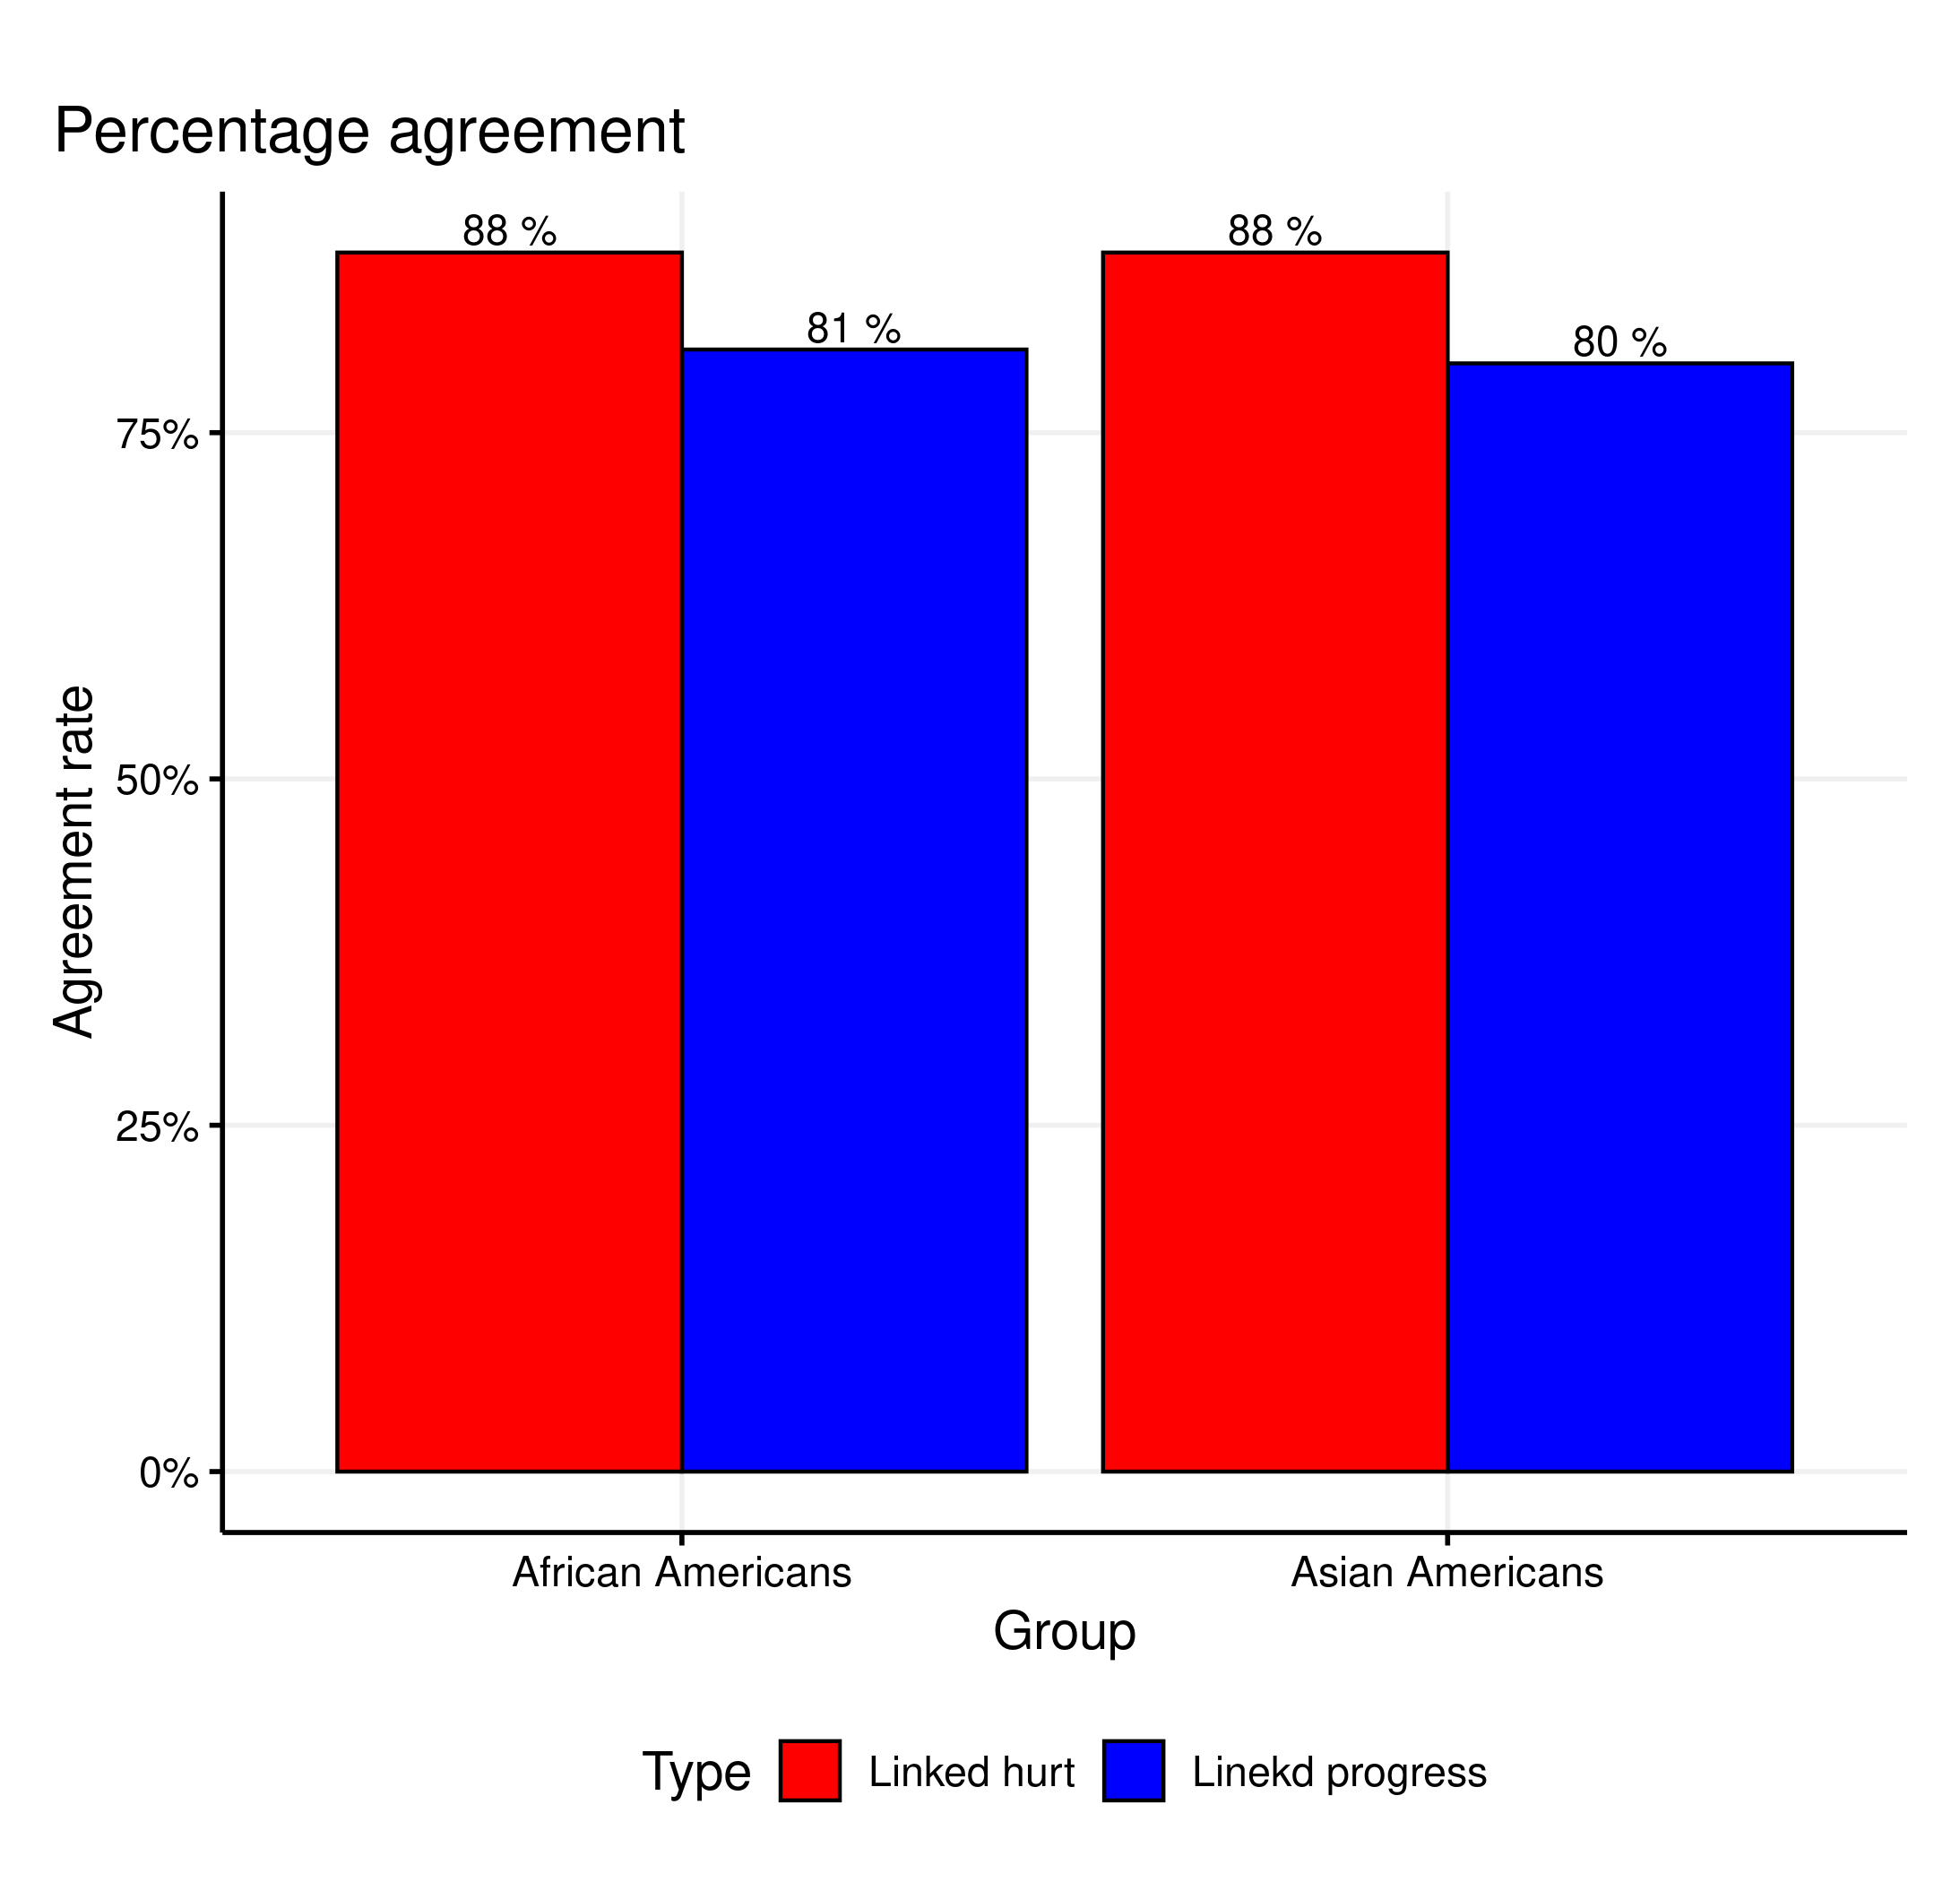
\includegraphics[width=0.6\linewidth]{content_analysis_agreement.png}
    \caption{Percentage agreement for linked progress and linked hurt articles}
    \label{fig:percentage_agreement}
\end{figure}

\subsection{Cohen's Kappa}

\begin{figure}[htbp!]
    \centering
    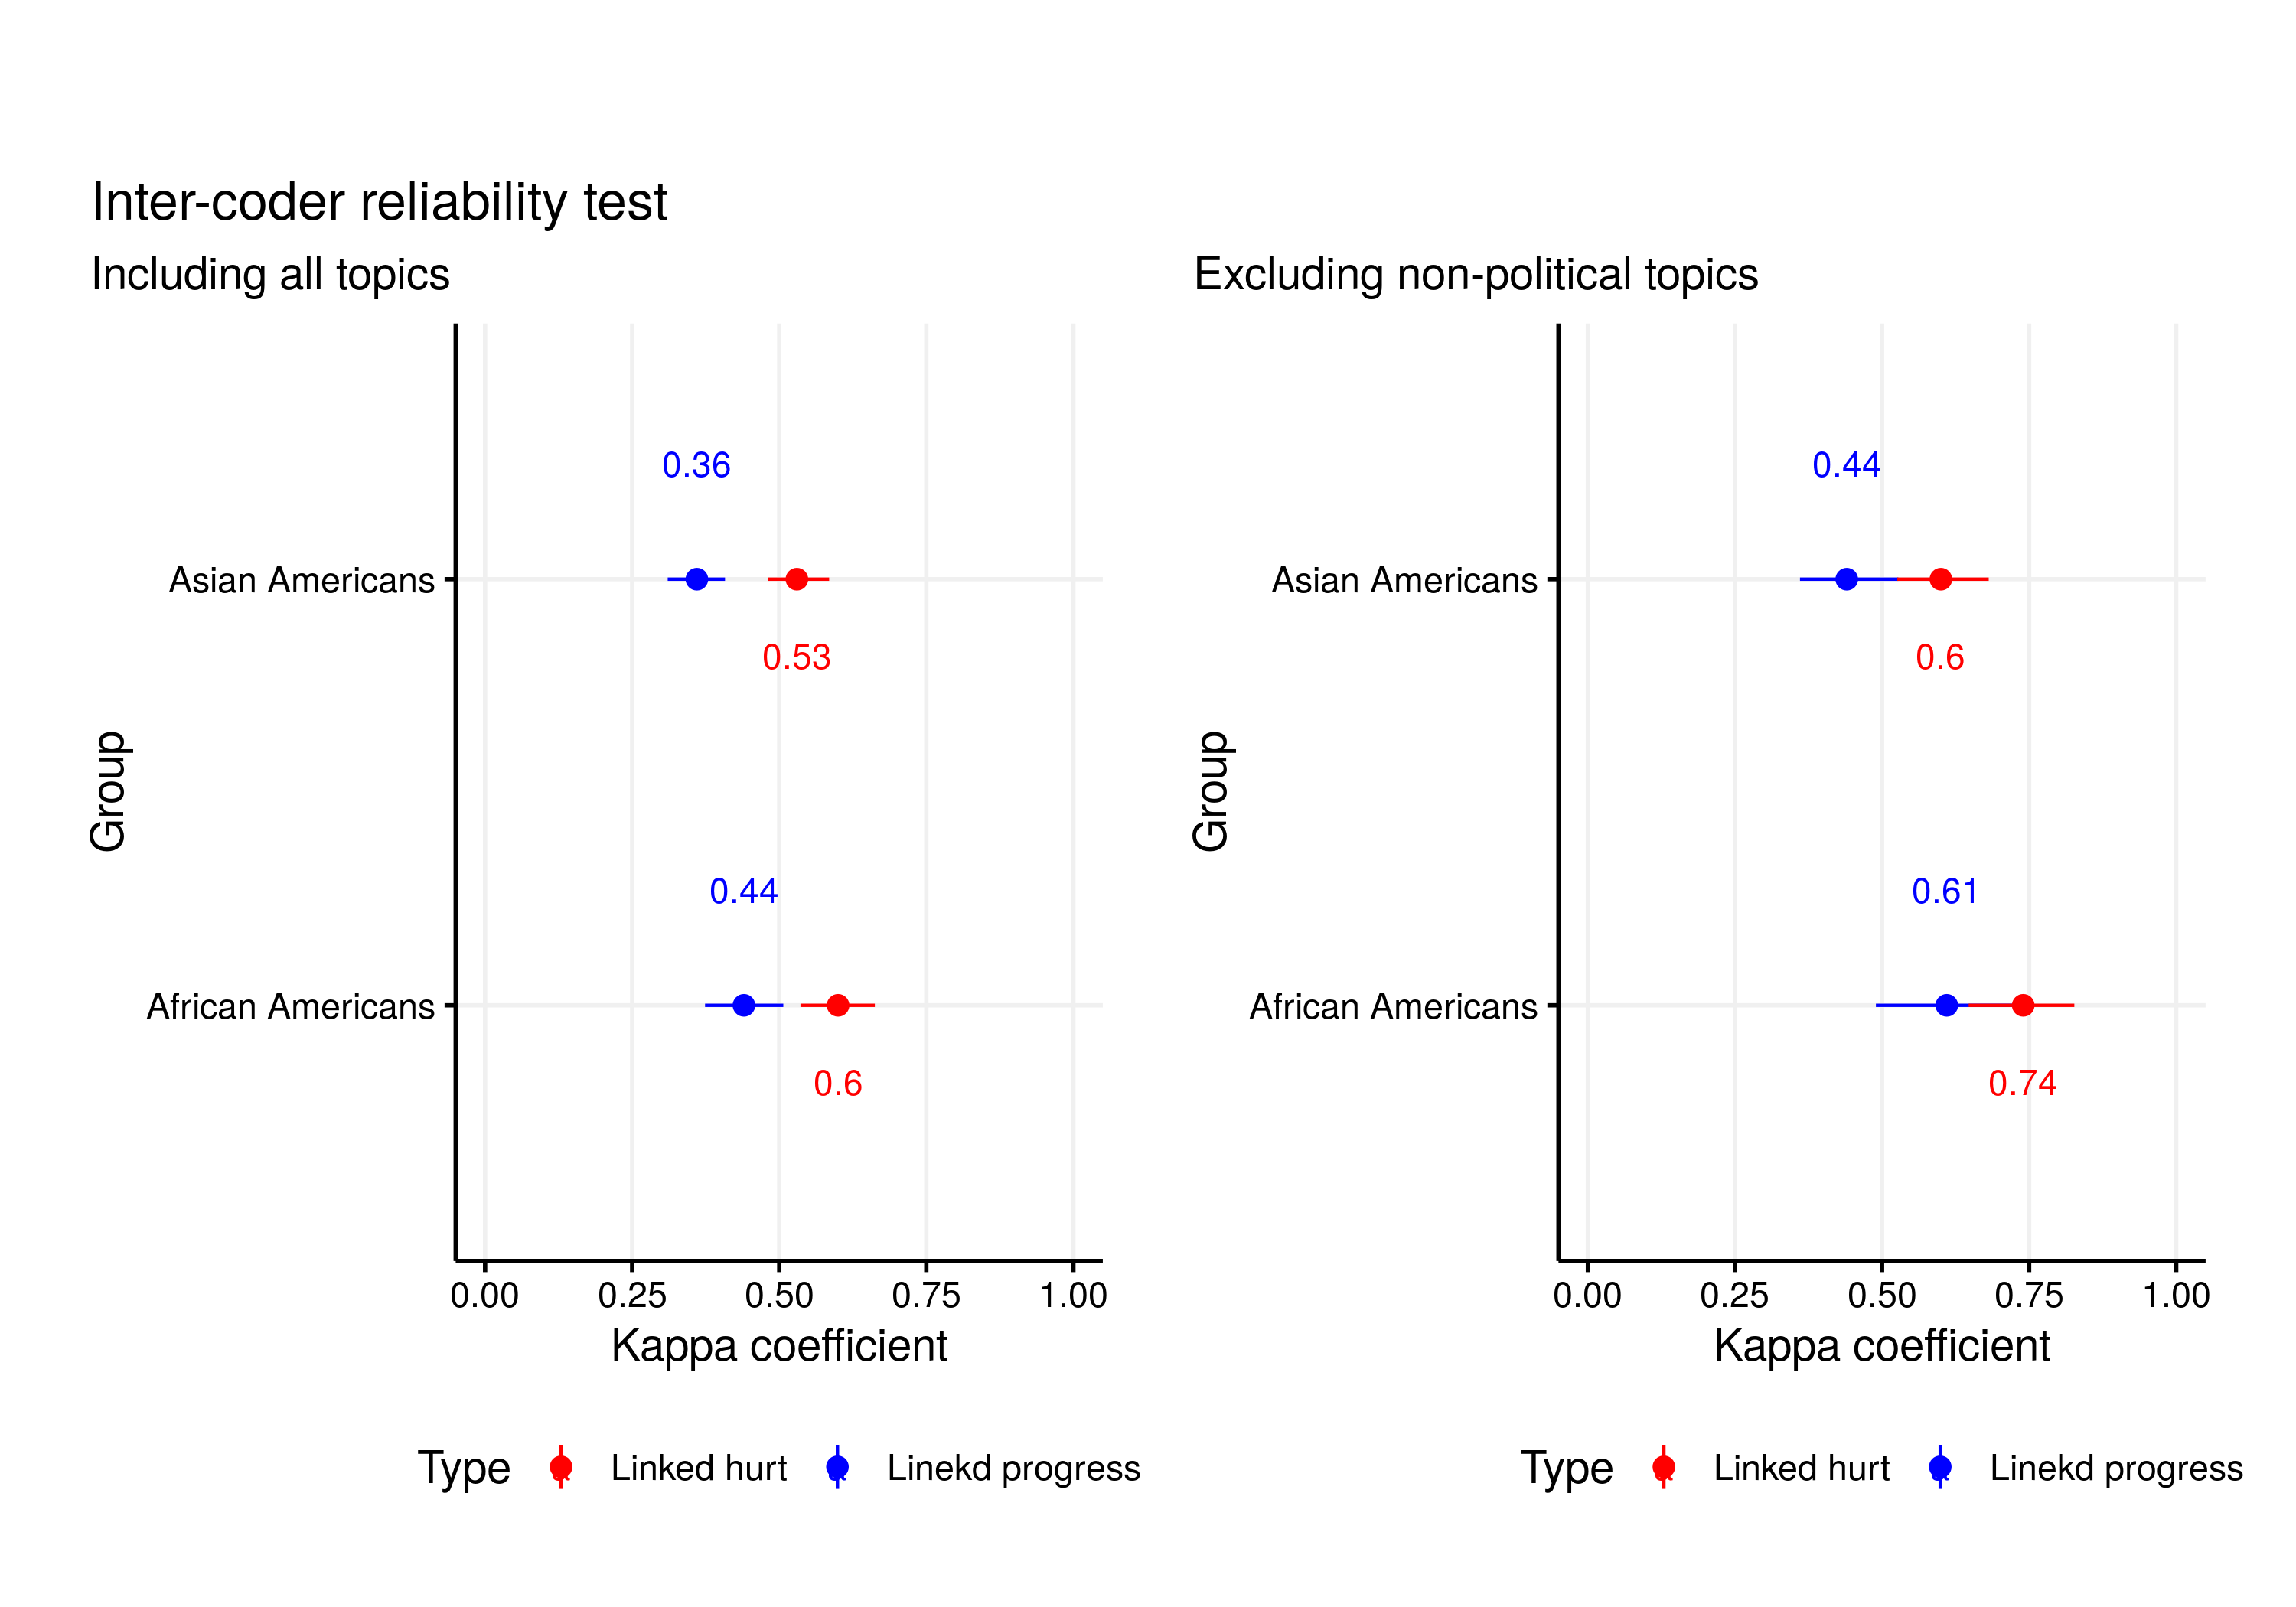
\includegraphics[width=0.9\linewidth]{content_analysis_kappa_comp.png}
    \caption{Cohen's kappa with or without non-political topics}
    \label{fig:cohen_kappa_comp}
\end{figure}

As the percentage agreement does not account for the stochastic element of the labeling process, it is time to turn to Cohen's kappa. The kappa score is relatively higher for the linked hurt articles in both newspapers (see the left panel in Figure \ref{fig:cohen_kappa_comp}). In addition, the labels in the African American newspapers are more reliable than those in their Asian American counterparts. Non-political issues, such as food and sports, could confuse human coders and increase disagreement between them. The right panel in the figure demonstrates how removing these articles increases inter-coder reliability. The results indicate that the training data are less reliable for non-political articles. Because unreliable data lead to weak prediction accuracy, I exclude non-political articles from the unlabeled data by using a dictionary method. The specific terms used to create the dictionary are listed in the Appendix \ref{appendix:dic}. 

\subsection{Construct Validity Test}

The next step is to check construct validity. So far, we have tested how reliably the human coders labeled the training data. Now, we turn to whether the measures really measure what they are designed to measure. The theory assumes that linked progress articles are likely to be associated with supportive government policies. By contrast, linked hurt articles are likely to be related to oppressive government policies. In Figure \ref{fig:construct_validity_test}, the X-axis is the difference between the number of linked progress articles and that of linked hurt articles belonging to the identical topic. The Y-axis indicates these topics. The red bar plot indicates that the maximum threshold is used to define linked progress and hurt labels. The blue bar plot indicates the use of the minimum threshold for the measurement. 

The analysis confirms that meta and specific issues hang together, as expected by the theory. This relationship holds regardless of whether one uses the maximum or minimum threshold to define the meta issues in the training data. In the figure, the topics strongly associated with linked progress articles are at the top, and the topics highly related to linked hurt articles are at the bottom. In the Asian American case, healthcare and political representation are the top two issues related to linked progress, and hate crimes and Asian stereotypes are the top two issues associated with linked hurt. After independent topic labeling, the human coders also provided a brief summary of each topic. Based on these summaries, on the Asian American side, healthcare was about the physical and mental well-being of people of Asian descent, which consisted of access to health education, health services, and availability of translators and translations to access these services. Political representation was about the potential increase in political engagement of Asian Americans in politics at the local, state, and federal levels, especially in gaining recognition in US Census data collection. Hate crimes were about instances of violence or discrimination against Asian Americans, and Asian American stereotypes were about generalizations of Asian men and women and cultural perceptions of outsiders as well as those within the Asian community. Issues about increasing government support were strong indicators of the linked progress articles, and issues about reducing outside threat, although not necessarily oppressive government policies, were leading signs of linked hurt articles. 

The African American newspaper follows the same pattern. School programs were about public school programs and administration in the San Francisco Bay Area. This issue was counted as a top issue related to linked progress articles. Criminal justice was about discrimination against African American defendants who were given unfair trials, legislators excluded from important committees, and citizens with higher imprisonment rates. Similarly, civil rights were about the overlapping topics of federal employees' failure (in terms of neglect of duty, abuse of power, or discrimination) and proposed laws, some of which would disproportionately affect African Americans. These were the top two issues related to linked hurt articles.

\begin{figure}[htbp!]
    \centering
    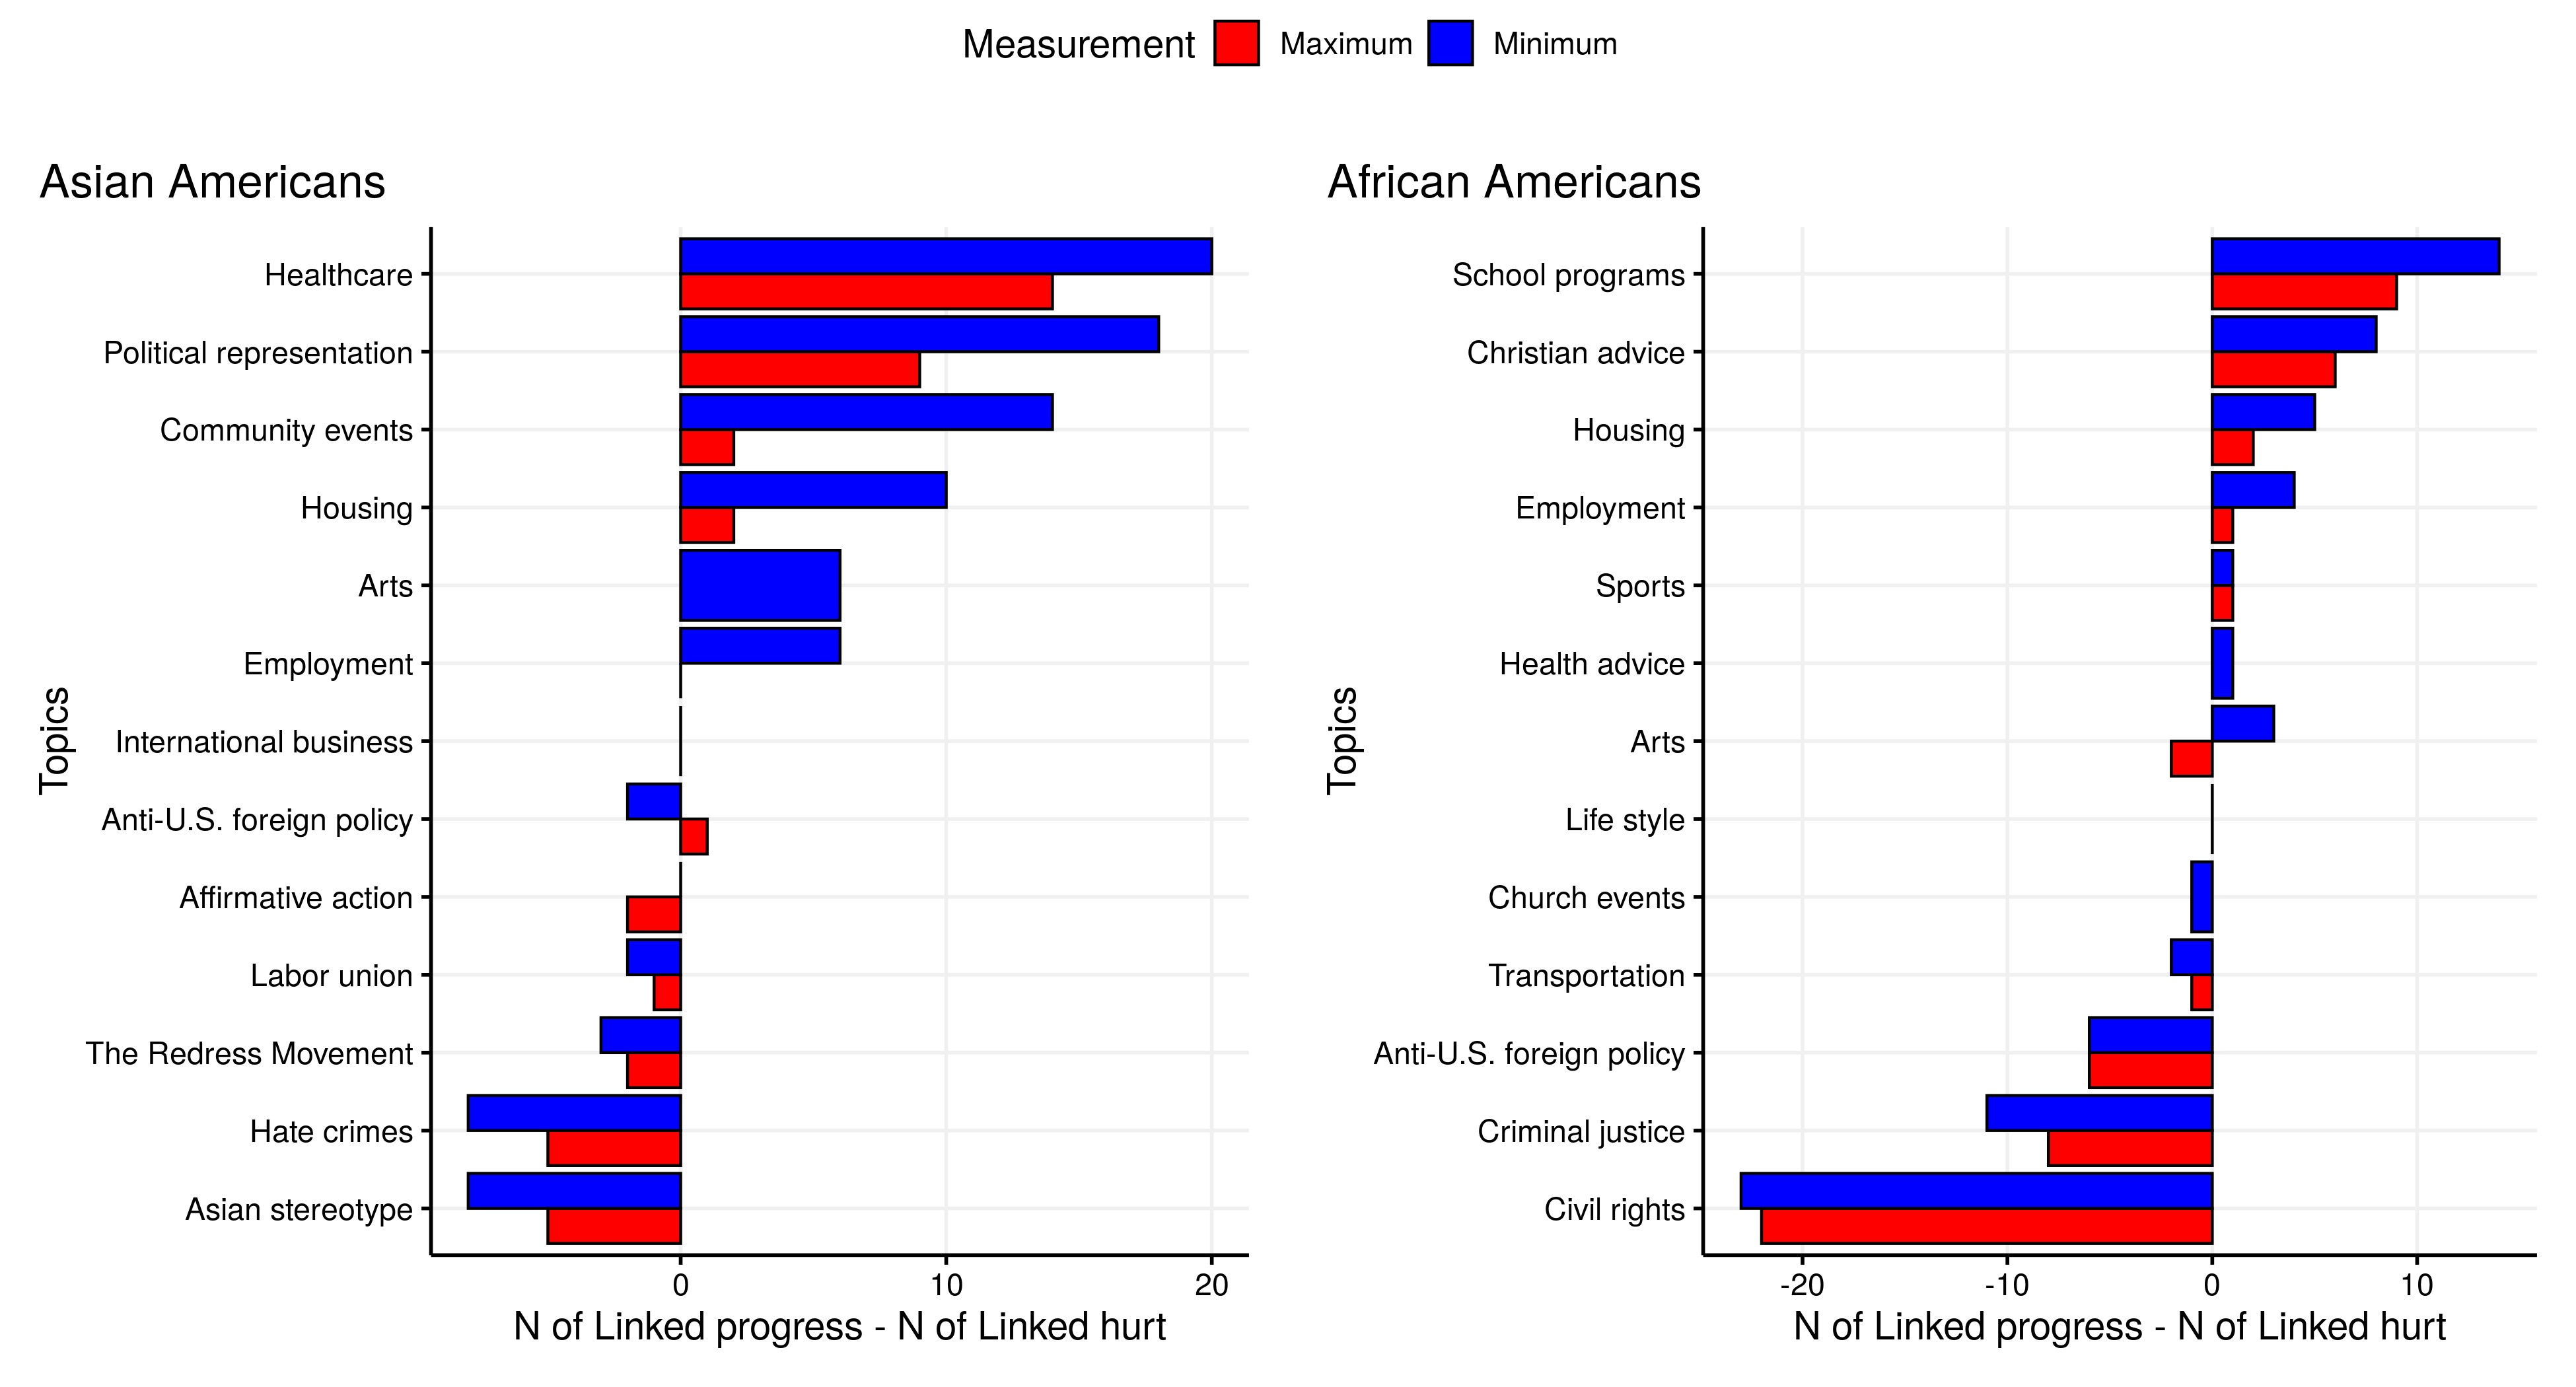
\includegraphics[width = 1\linewidth]{content_analysis_topics_gran.png}
    \caption{Construct validity test}
    \label{fig:construct_validity_test}
\end{figure}

\begin{figure}[htbp!]
    \centering
    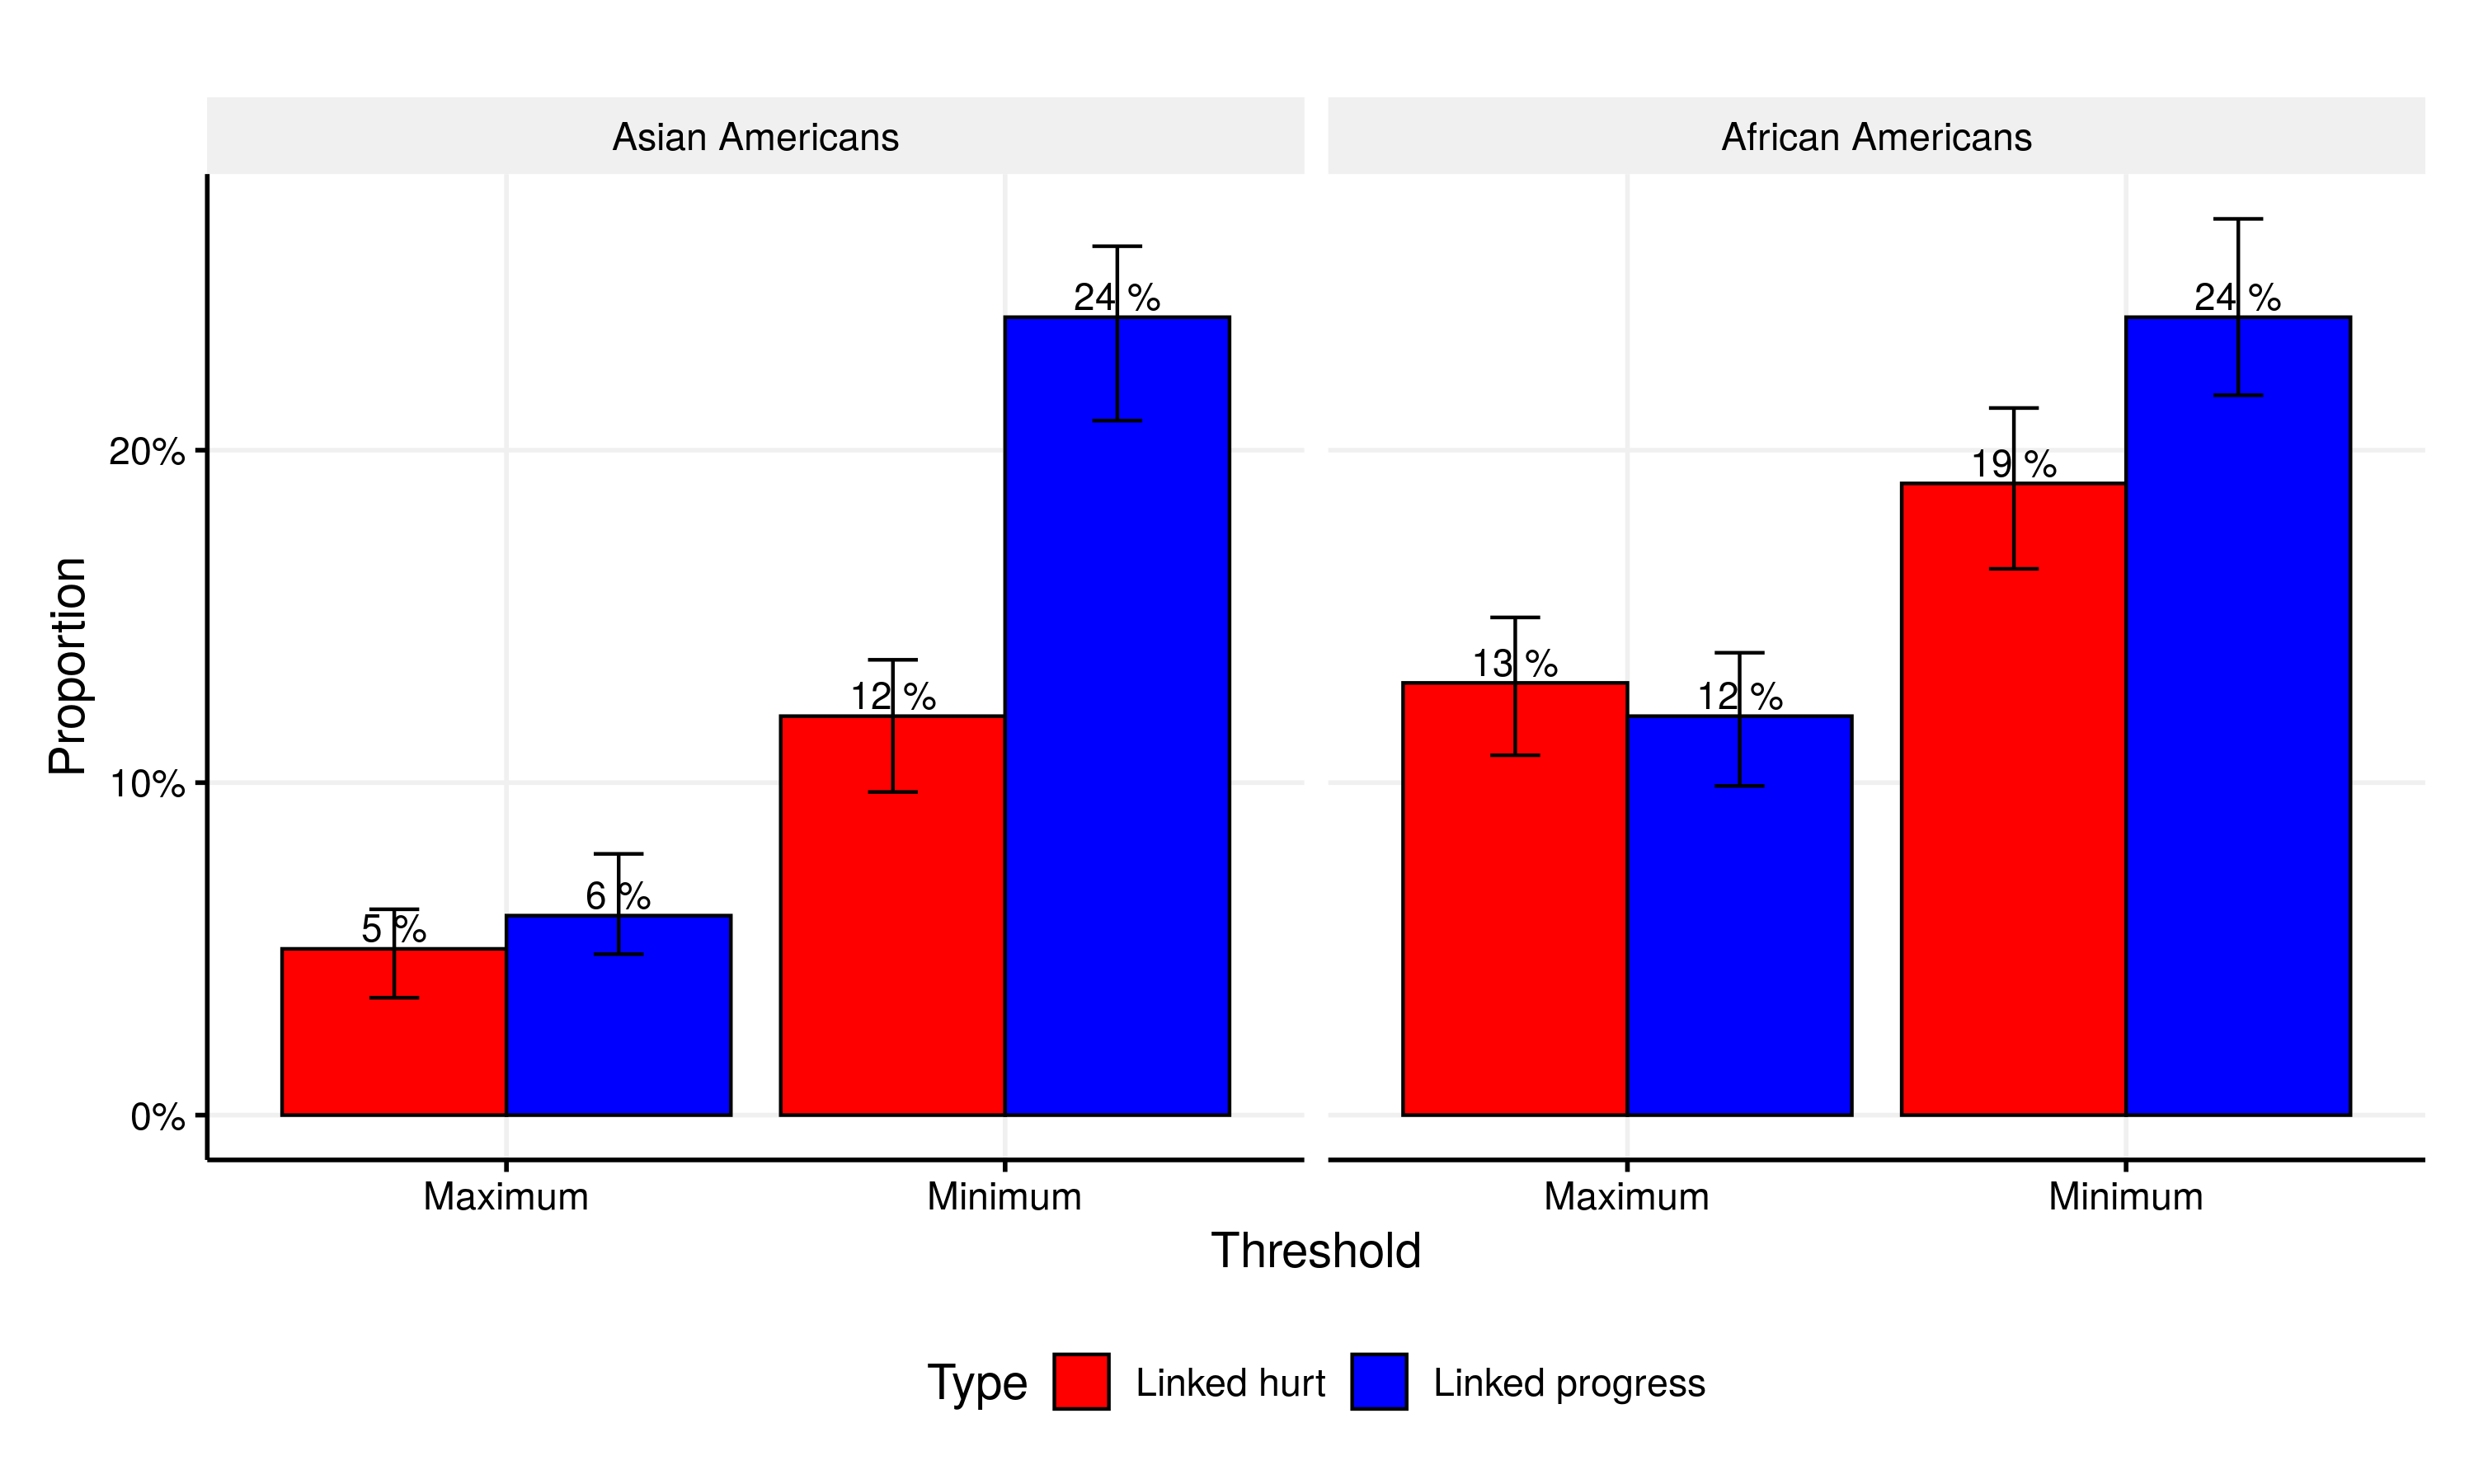
\includegraphics[width=0.9\linewidth]{content_data_sources_sub.png}
    \caption{Threshold change and the proportion of linked progress and hurt articles}
    \label{fig:content_case_proportion}
\end{figure}

One noticeable difference between the two groups is the extent to which the threshold change affects the proportion of linked progress and hurt articles. As Figure \ref{fig:content_case_proportion} illustrates, using the maximum threshold increases the proportion of linked progress articles by 300\% and that of linked hurt articles by 140\% in the Asian American corpus. The same change moves up the proportion of linked progress articles by 200\% and that of linked hurt articles by 46\% in the African American corpus. Overall, the Asian American corpus displays a greater degree of variability. This pattern is expected because the labels in the Asian American corpus are less reliable than their African American counterparts on the basis of their kappa scores (see Figure \ref{fig:cohen_kappa_comp}). The content of the labels changes little regardless of whether the training data are measured by the minimum or the maximum threshold. Nevertheless, the asymmetry in the class size variation implies that the impact of the threshold change on the predicted labels would be disproportionately high for the Asian American corpus compared with the African American one.

\section{Text Classification}
Automated text classification scales up content analysis using machine learning. In Figure \ref{fig:ml_performance_evaluation}, the X-axis indicates the accuracy or the balanced accuracy rate. The Y-axis indicates different classifiers. The dotted lines represent the percentage agreement between the human coders. The figure demonstrates that more reliable and balanced data produced better prediction outcomes. The worst performance is found in the bottom left panel, where the training data are measured by the minimum threshold and no resampling is used. The average accuracy rate is 77\%, but the average balanced accuracy rate is 63\%. The best performance is found in the top right panel, where the training data are measured by the maximum threshold and upsampling is used. The average accuracy rate goes up by 19\%, and the average balanced accuracy rate moves up by 32\%. Both Lasso and XGBoost exhibit similar high performance. However, when these classifiers were used to predict the unlabeled data, XGBoost did not perform well. For example, when the training data were measured by the maximum threshold and upsampled, the algorithm was able to classify only four Asian American and 171 African American linked hurt articles. This prediction is likely a strong underestimate of the true count of linked hurt articles. For instance, hate crimes are a strong indicator of linked hurt articles among Asian American newspapers (see Figure \ref{fig:construct_validity_test}). Asian American newspapers all highlighted how an anti-Asian attitude led to the murder of Vincent Chin. \textit{Asian Week} covered the Vincent Chin case 212 times and \textit{International Examiner} 40 times between April 1983 and December 1989. These articles argued that Vincent Chin's murder was a hate crime. Even if we only counted these articles, the number of relevant cases for linked hurt should be 63 times larger than the predicted estimate. I selected Lasso to classify the unlabeled data because it demonstrated the most stable high performance.

\begin{figure}[htbp!]
    \centering
    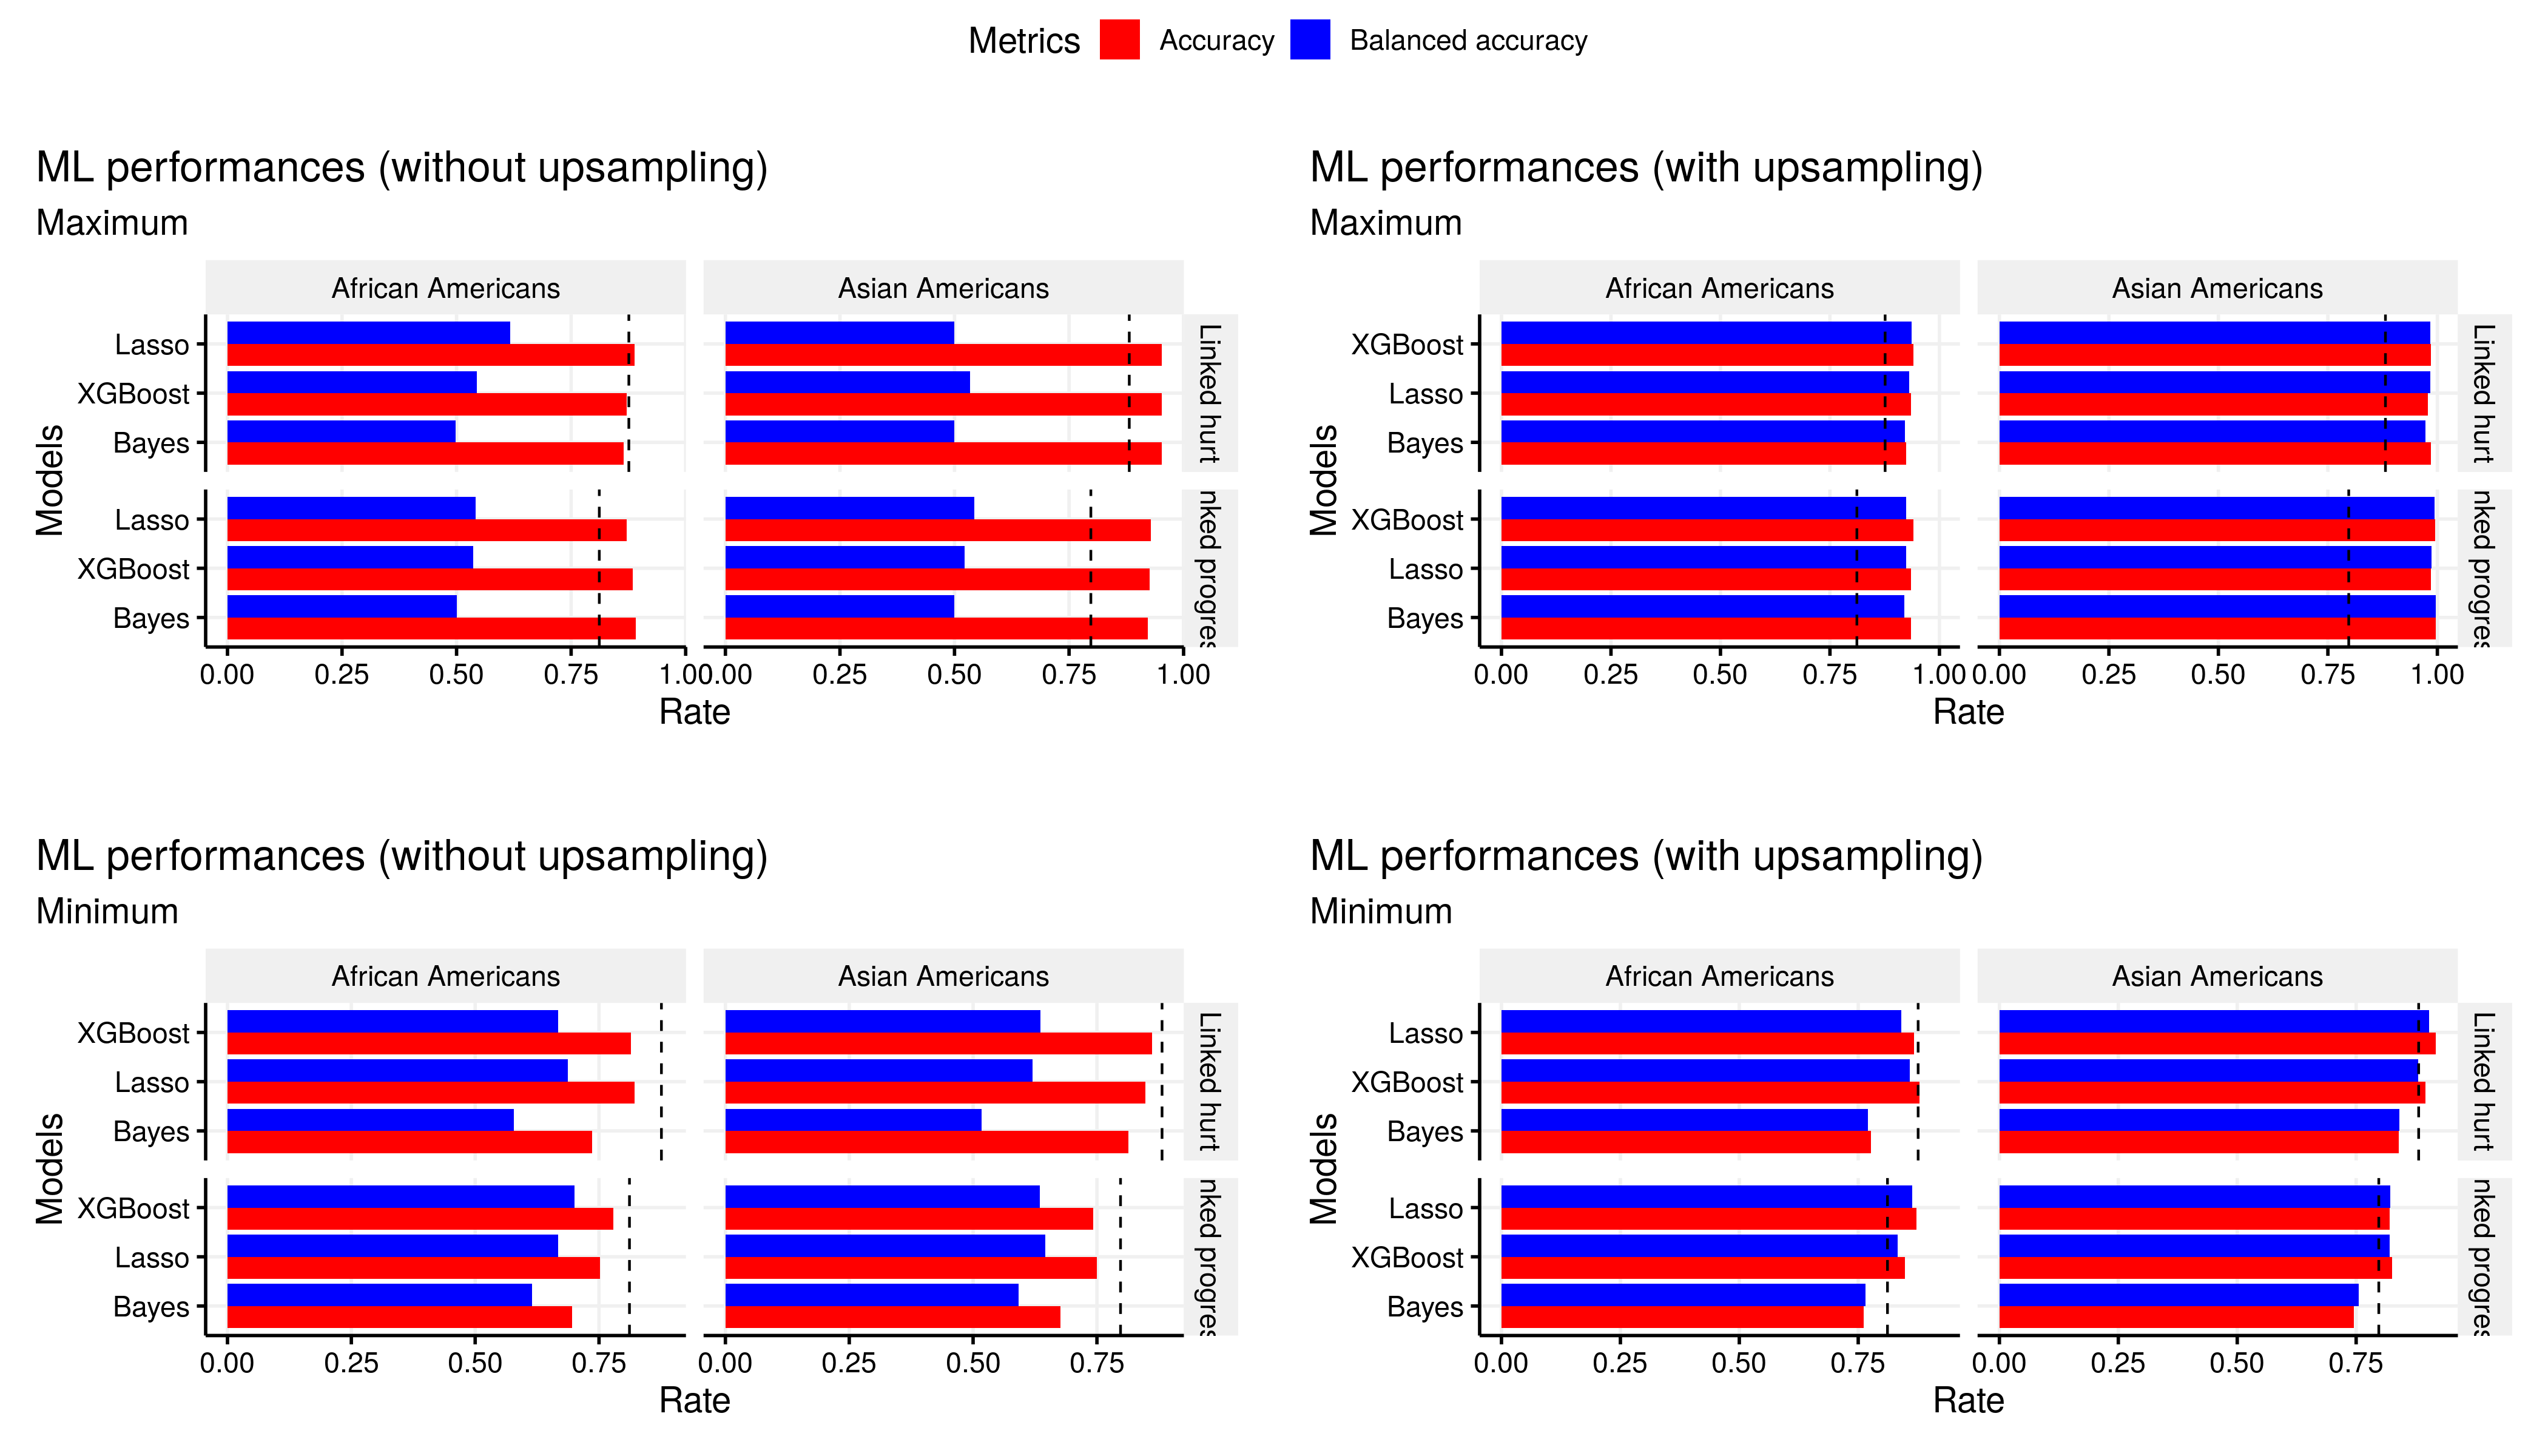
\includegraphics[width=1\linewidth]{ml_content_comp.png}
    \caption{Classifier performance evaluations}
    \label{fig:ml_performance_evaluation}
\end{figure}

Data quality affects not only prediction accuracy but also substantive results. Figure \ref{fig:ts_max} displays how the proportion of linked progress and hurt articles varies between the two groups over time. In this case, the training data are measured by the maximum threshold. The Y-axis shows the percentage of articles in the corpus classified as the given meta issue type, and the X-axis indicates either publication years or months. The ribbons indicate 95\% confidence intervals. The blue line indicates the proportion of exclusive linked progress articles, the red line indicates the proportion of exclusive linked hurt articles, and the purple line indicates the proportion of articles classified as both linked progress and hurt. Overall, the blue line is above the red line in the Asian American case, and the pattern is reversed in the African American case. Put differently, Asian American newspapers issued linked progress articles far more frequently than linked hurt articles. This pattern is reversed in the African American case. 

\begin{figure}[htbp!]
    \centering
    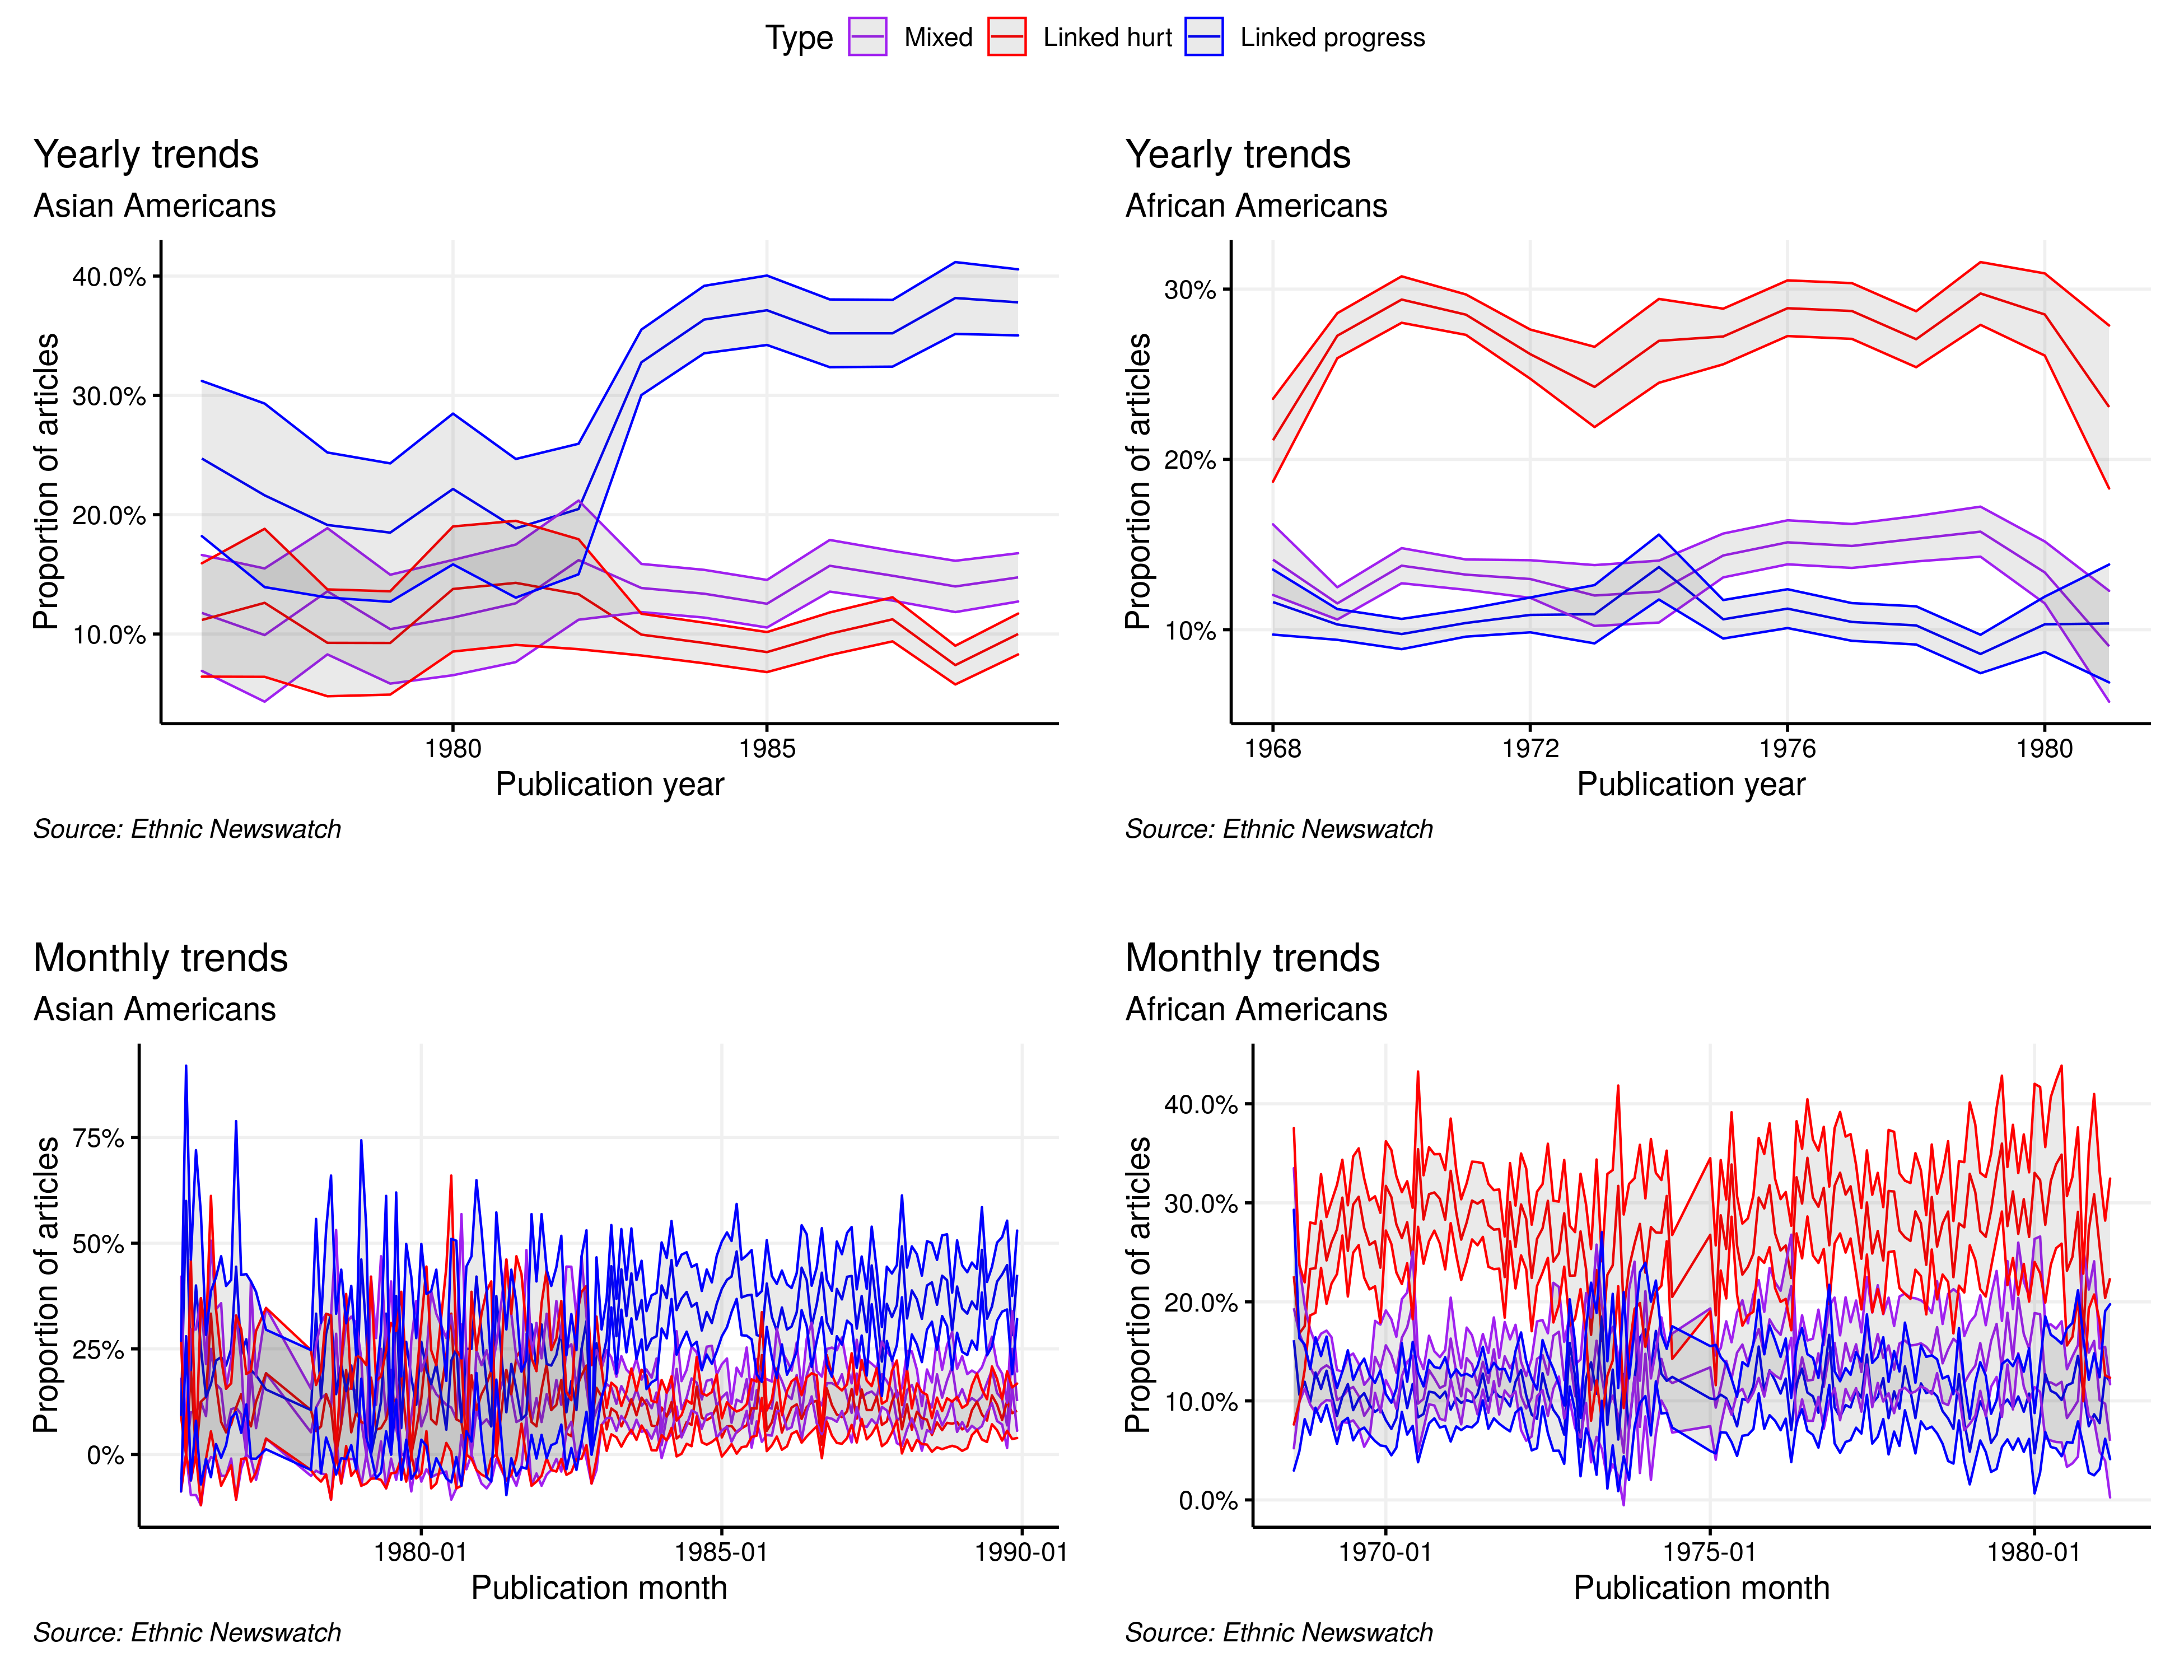
\includegraphics[width=0.8\linewidth]{time_series_plot.png}
    \caption{Time series trends (maximum threshold)}
    \label{fig:ts_max}
\end{figure}

\begin{figure}[htbp!]
    \centering
    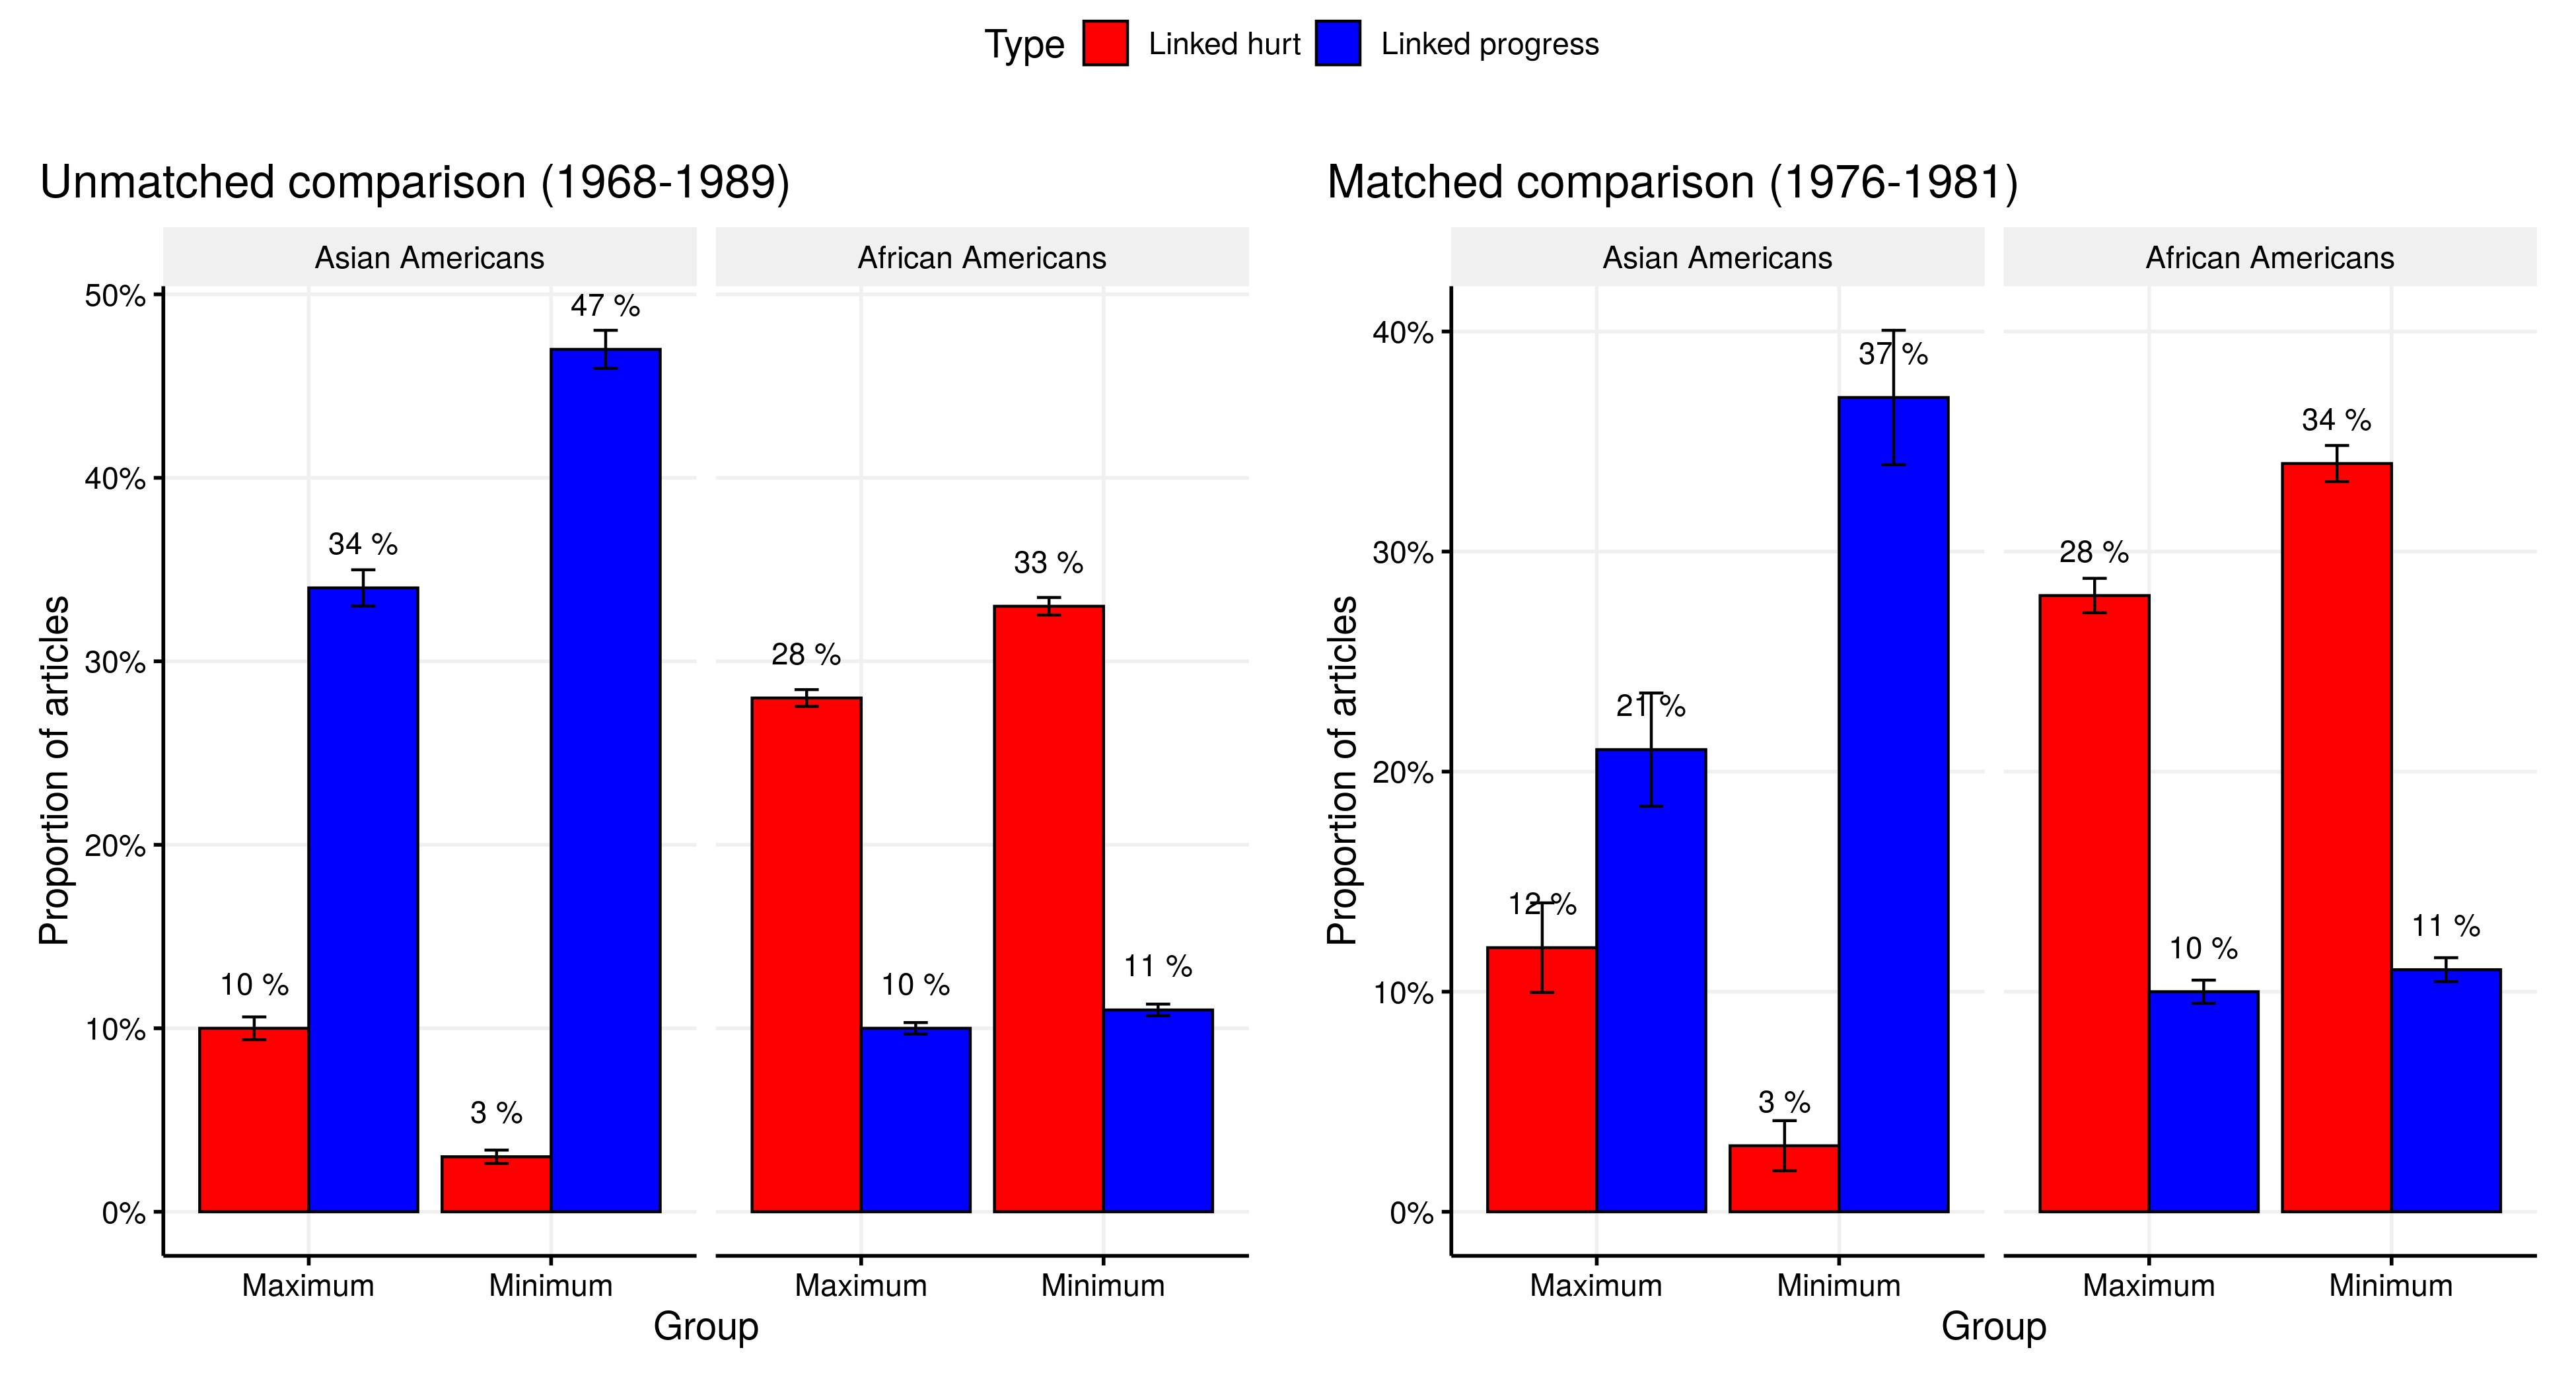
\includegraphics[width=1\linewidth]{matched_comparison_year.png}
    \caption{How text classification is sensitive to measurement decisions}
    \label{fig:ts_unmatched}
\end{figure}


The contrast between the groups can be more closely examined using bar plots. I also dropped the mixed category to make the comparison simple. In Figure \ref{fig:ts_unmatched}, the X-axis is the group, and the Y-axis is the proportion of linked progress and hurt articles. The publication years in the Asian American and African American corpora do not precisely match. The Asian American corpus was collected from 1976 to 1989 and the African American corpus from 1968 to 1979. To show whether this difference matters for comparison, I matched the two data on their publication years in the right panel and did not do the same in the left panel. In both panels, Asian American newspapers clearly preferred linked progress, whereas African American newspapers preferred linked hurt. The errors bars represent 95\% confidence intervals. As the height differences between the bar plots are much greater than these intervals, it is easy to see that these differences are statistically significant. To be precise, I calculated the differences in the proportions of linked progress and hurt articles between the Asian American and African American corpora. Matching the two corpora decreases the gap between the two groups. In the following measures, the lower range comes from the matched data and the upper range comes from the unmatched data. The data show that Asian American newspapers issued linked progress articles by 110\%-240\% more than African American newspapers did. By contrast, African American newspapers produced linked hurt articles by 133\%-180\% more than their Asian American counterparts did. Measuring the training data by the minimum threshold widens the gap between the two groups. When the threshold shifted to the minimum, Asian American newspapers reported on linked progress up to three times more than African American newspapers did. By contrast, African American newspapers covered linked hurt up to 10 times more than their Asian American counterparts. As Figure \ref{fig:ts_unmatched} shows, note that the extreme difference was driven by Asian American newspapers. Less reliable training data lead to more extreme interpretations. 

Finally, some unstable patterns deserve further explanations. In Figure \ref{fig:ts_max}, the proportion of linked progress articles in Asian American corpus surged in the early 1980s. This increase is a likely result of combining two different data sources. Figure \ref{fig:ts_max_source} in the Appendix \ref{appendix:ts_plots} shows that the proportion of linked progress articles is higher in \textit{Asian Week} than in \textit{International Examiner}. This difference does not simply derive from the fact that their publication years are different. Even if we matched the two newspaper data on their publication years (1983-1987), the average proportion of linked progress articles in \textit{Asian Week} is 40\% greater than the same measure in \textit{International Examiner}. The two data sources were combined in the time series plot starting in 1983, and this explains the abrupt increase in the proportion of linked progress articles appearing around that cutpoint. In addition, this surging trend seems conditional on the measurement decision, as it does not appear when the training data are measured by the minimum threshold (see Figure \ref{fig:ts_min_source} in the Appendix \ref{appendix:ts_plots}).

\section{Discussions and Conclusion}
Textual data are attractive because they allow political scientists to analyze the words of politicians and citizens---the content of democracy \citep[311]{brady2019challenge}. Nevertheless, the application of the method has been uneven, as most cases are limited to the study of the words of the powerful, such as US Congress members \citep{hopkins2010method, grimmer2012words}. The voice of marginalized members has rarely been systematically examined. This study fills such a gap by setting an example of how we can apply machine learning to investigate how political issues vary among ethnoracial minority groups over time.

The findings demonstrate why careful and systematic content analysis is essential for automated text classification. Content analysis is labor intensive. More importantly, although the content analysis is based on a probability sample, the descriptive statistics drawn from the analysis are still prone to error, as the sampling variance is unknown. Automated text classification is an efficient alternative to this traditional method, as machine learning algorithms can label a large collection of documents at an impressive speed. In addition, sampling variance is no longer a concern, as the analysis is based on the entire corpus. Nevertheless, a healthy dose of skepticism is still useful in embracing this new method. Uncertainty exists regarding how machine learning algorithms predict labels and how researchers can interpret the results. The findings clearly illustrate that unreliable training data lead to not only weak predictions but also extreme interpretations. When the maximum threshold was used to label the training data, the difference in issue priorities between Asian Americans and African Americans was moderate. When the maximum threshold was used, the gap between the two groups widened up to 10 times. 

Although purely descriptive, the original large-scale evidence provides new insights into why building an interracial coalition has been difficult in the US. A theory is built upon the descriptions of the real world that it aims to model. If the descriptions change, the theory should also change. The findings show that from a relative perspective, whereas the African American corpus focused on opposing state oppression, the Asian American corpus concentrated on expanding state support. Ethnoracial minorities are often collectively labeled as people of color because they share racial marginalization. Race is not just all about the color of one's skin, but it is a social construct often created by an oppressive historical process \citep{omi_racial_1994}. Nevertheless, sharing the experience of marginalization is often insufficient to foster coalition among minority groups. Past studies also acknowledge that group commonality might be a necessary but not sufficient condition for the formation of interracial coalitions \citep[201]{kaufmann2003cracks}. However, the literature has been elusive about the missing element. This study identified one of the potentially missing mechanisms by focusing on the rarity of Black-Asian coalitions in the West Coast in the 1960s and 1970s. Given their strong social and political connections, these groups were natural coalition partners. Despite these connections, these groups faced difficulties in forging a coalition because they had different issue priorities based on different kinds of policy challenges they needed to deal with. This claim is not entirely novel, as historians have already pointed out that marginalization, which political scientists often operationalized as the perception of discrimination, is a crude measure to capture how minority groups strategically approached the challenge of forming interracial coalitions. For instance, \citet[210]{brilliant2010color} argued that different racial minority groups were affected by “different axes of discrimination” and therefore used “different avenues of legal and legislative redress.” From a distant perspective, the issues of non-White groups seemed similar, as they were rooted in the fact that such groups were disadvantaged in US society. However, taking a close look at their issues, we realized that the two groups ranked their main issues in different ways because different racial groups had to deal with different policy challenges. I build and expand on this insight from the historical scholarship by providing a novel conceptual and methodological framework. The findings encourage scholars to measure racial marginalization more carefully, especially in policy terms, to estimate the cost of coordinating among ethnoracial groups more accurately. 

\clearpage

\printbibliography

%\clearpage % Ensure all floats are processed
%\processdelayedfloats
%\clearpage

%\makeatletter
%\efloat@restorefloats
%\makeatother

\clearpage
\counterwithin{figure}{section} 
\counterwithin{table}{section}

\begin{appendices}

\section{Custom Dictionary for Non-political Issues}
\label{appendix:dic}

\begin{itemize}
\item Sports: "football", "basketball", "golf", "tennis", "swimming", "coach", "giants", "warriors", "raiders", "49ers", "track team", "track and field", "athletes", "soccer"
\item Car sales: "engine", "powersteering", "windshields", "gasoline", "motors", "subcompact", "showrooms", "fuel prices" 
\item Arts: "art", "arts", "film", "films", "museum", "galleries", "painting", "paintings", "theater", "television", "circus", "opera", "orchestra", "symphony", "jazz", "disco", "concert", "concerts", "festival", "festivals", "artists", "artist", "singer", "musician", "musicians", "pianist", "pianists", "guitarists", "guitarist", "ticket", "tickets", "violin", "lion dance"
\item Recipes and restaurants: "recipe", "lunch", "lunch special", "dinner", "dinners", "entrees", "breakfast", "cooking", "teaspoon", "teaspoons", "quarts", "tablespoon", "tablespoons", "sugar", "fried"
\end{itemize}

\clearpage

\section{Time Series Plots}
\label{appendix:ts_plots}

\begin{figure}[htbp!]
    \centering
    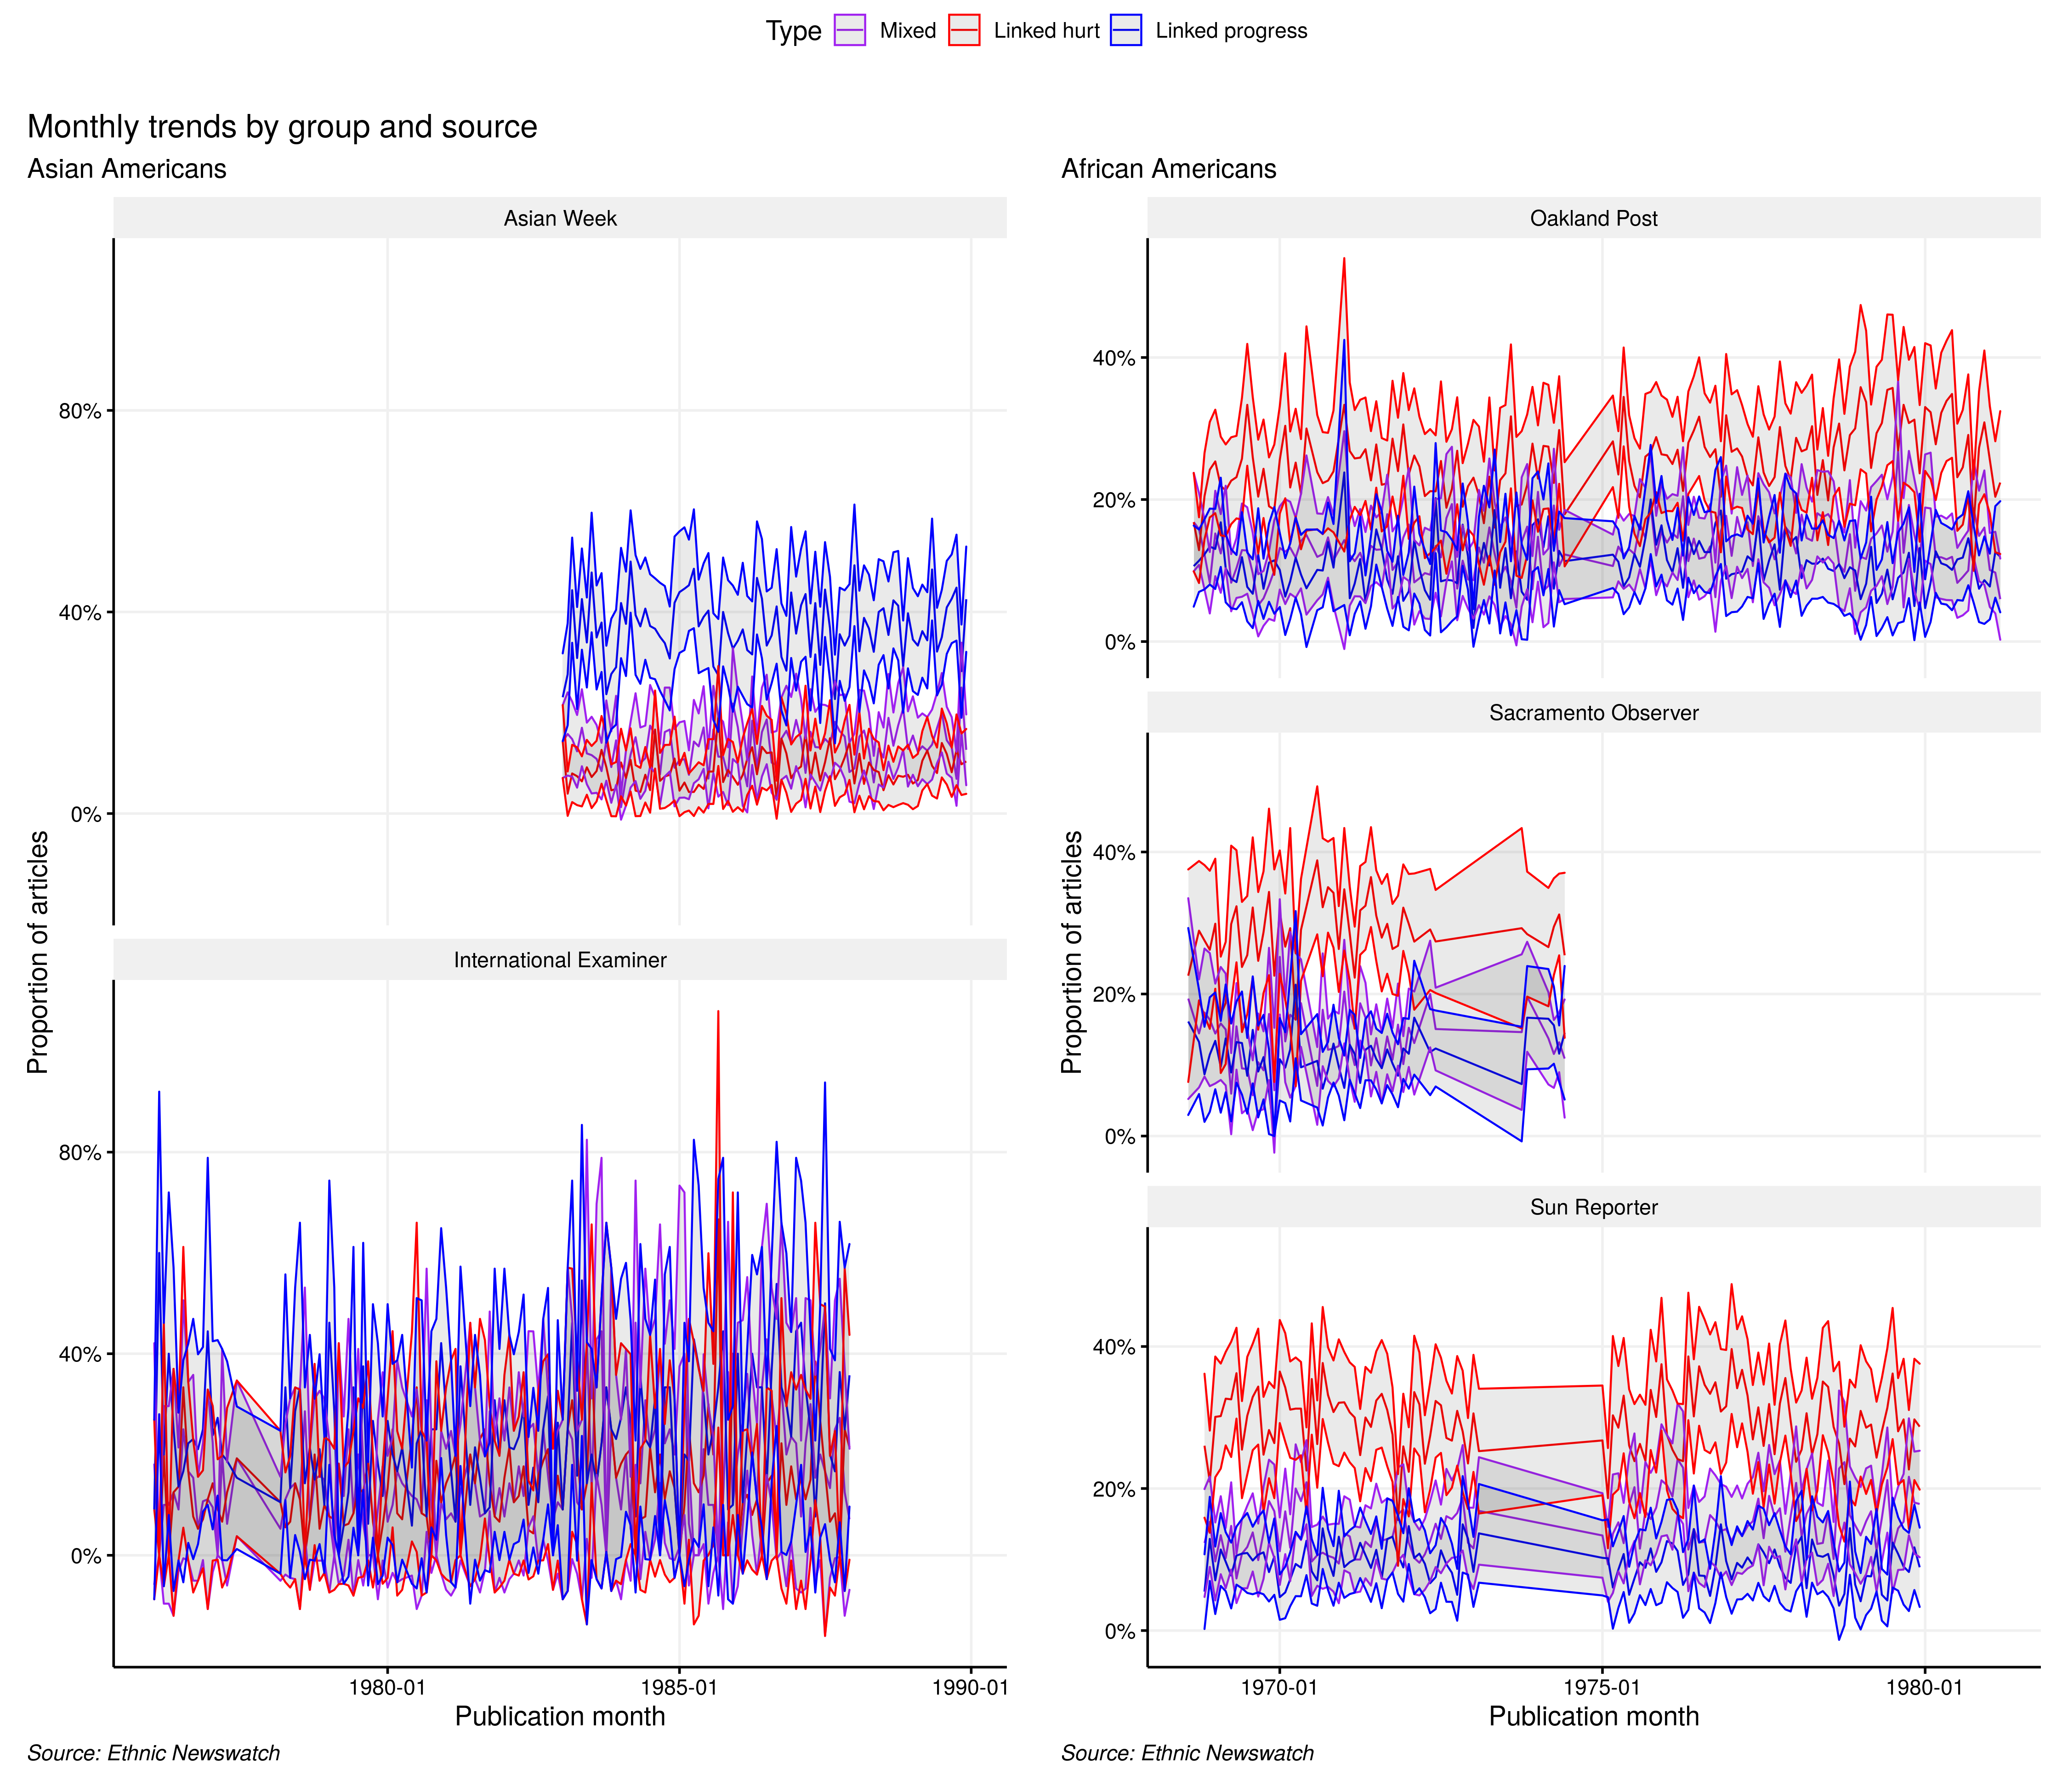
\includegraphics[width=0.8\linewidth]{time_series_source.png}
    \caption{Time series trends (maximum threshold)}
    \label{fig:ts_max_source}
\end{figure}

\begin{figure}[htbp!]
    \centering
    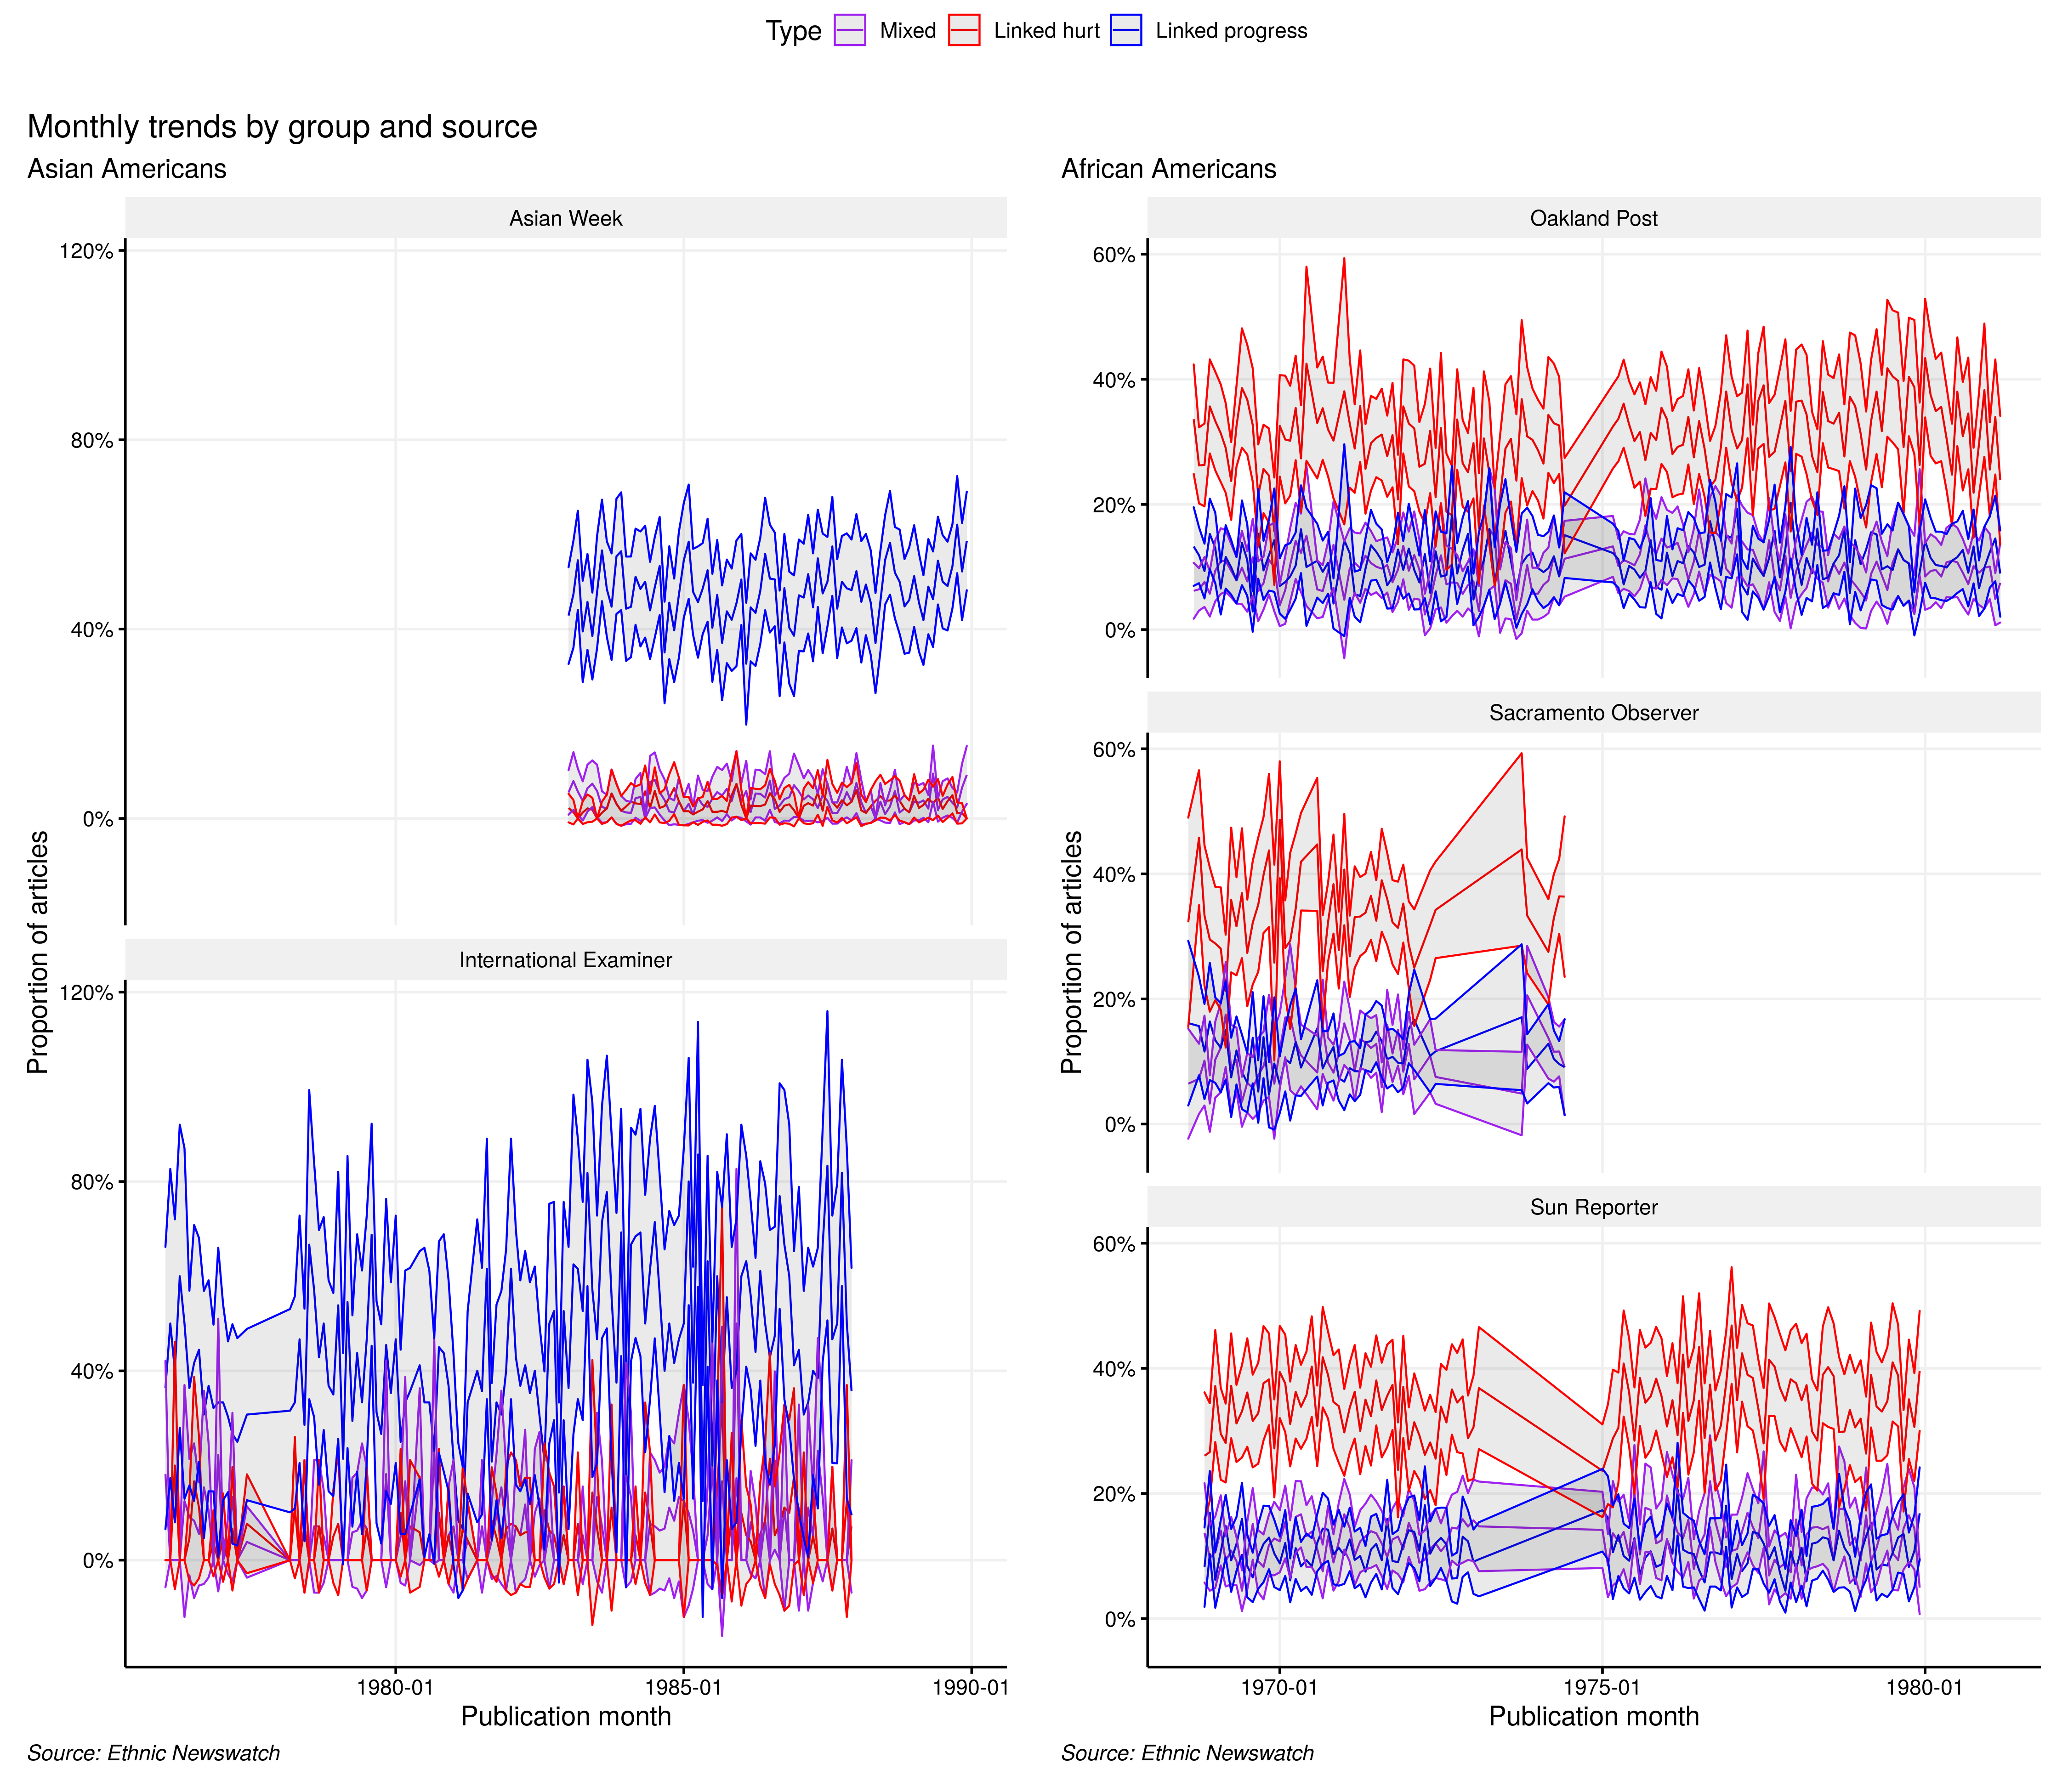
\includegraphics[width=0.8\linewidth]{time_series_source_gran.png}
    \caption{Time series trends (minimum threshold)}
    \label{fig:ts_min_source}
\end{figure}

\clearpage

\end{appendices}

\end{document}